\documentclass[article,final,14pt]{scrreprt}
\usepackage[utf8x]{inputenc}
\usepackage[russian]{babel}
\usepackage{amsfonts}
\usepackage{amsthm}
\usepackage{amssymb}
\usepackage{vmargin}
\usepackage{amsmath}
\usepackage{graphicx}
\usepackage{listings}
\usepackage{color}
\usepackage{multicol}
% \usepackage[Lenny]{fncychap}
\usepackage{xcolor}
\usepackage{hyperref}
\setpapersize{A4}
\setmarginsrb{2cm}{1.5cm}{1cm}{1.5cm}{0pt}{0mm}{0pt}{13mm}
\usepackage{indentfirst}
\sloppy
\DeclareGraphicsExtensions{.pdf,.png,.jpg}
\graphicspath{{images/}}

\definecolor{linkcolor}{HTML}{800000}
\definecolor{urlcolor}{HTML}{6495ED}

\hypersetup{pdfstartview=FitH,  linkcolor=linkcolor,urlcolor=urlcolor, colorlinks=true}

\setcounter{tocdepth}{2}
\linespread{1}

\begin{document}

\newtheorem{theorem}{Теорема}

\newtheorem{problem}{Задача}[chapter]

\newtheorem{lemma}{Лемма}[chapter]

\newtheorem{clair}{Утверждение}[chapter]

\newtheorem{definition}{Определение}[chapter]

\newtheorem{property}{Свойство}[chapter]

\newtheorem{conseq}{Следствие}[chapter]

\newtheorem{properties}{Свойства}[chapter]

\newtheorem*{remark}{Замечание}

\newenvironment{Proof}       
	{\par\noindent{\bf Доказательство.}}
	{\hfill$\blacksquare$}

\newenvironment{solution}       
	{\par\noindent{\bf Решение.}}
	{\hfill$\blacksquare$}

\newcommand{\red}[1]{\textbf{\color{red}#1}}
\newcommand{\blue}[1]{\textbf{\color{blue}#1}}
\newcommand{\green}[1]{\textbf{\color{green}#1}}

\def\ton#1{1,2,\dots,#1}
\def\Set#1#2{\left\{#1\colon#2\right\}}
\def\MYdef{\mathrel{\stackrel{\rm def}=}}

\addto\captionsrussian{\def\refname{Список используемой литературы}}

\begin{titlepage}
  \begin{center}
    \large
 
 	МОСКОВСКИЙ ГОСУДАРСТВЕННЫЙ УНИВЕРСИТЕТ ИМЕНИ М. В. ЛОМОНОСОВА

    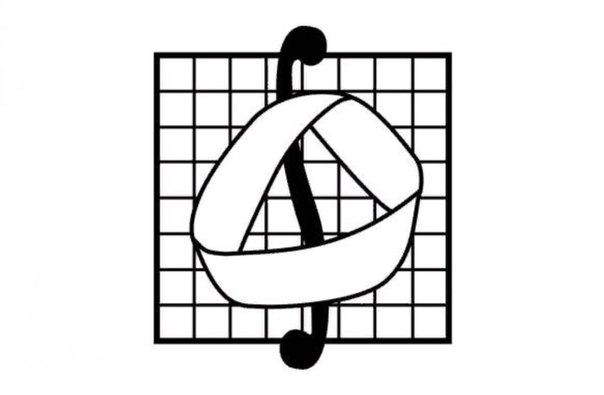
\includegraphics[scale=0.6]{mm.jpg} 
     
    Механико-математический факультет
    \vspace{0.25cm}

    Кафедра Вычислительной Математики
    \vspace{0.25cm}
 
    \textsc{Курсовая работа}\\[5mm]
     
    {\LARGE Восстановления отрезка по проекциям на плоскостях}
    \bigskip

    Конов Марк Андреевич
    \vspace{0.25cm}
     
    3 курс, группа 332
\end{center}
\vfill
 
\newlength{\ML}
\settowidth{\ML}{«\underline{\hspace{0.7cm}}» \underline{\hspace{2cm}}}
\hfill\begin{minipage}{0.5\textwidth}
  \begin{flushright}
     Научный руководитель\\
    к.ф.-м.н. \\
    Валединский Владимир Дмитриевич\\
    «\underline{\hspace{0.7cm}}» \underline{\hspace{2cm}} 2021 г.
  \end{flushright}
\end{minipage}%
\vfill
\bigskip
 
\begin{center}
  Москва, 2021 г.
\end{center}
\end{titlepage}
\newpage

\tableofcontents

\chapter{Постановка задачи}\label{task}

Даны три множества из $n_1$, $n_2$ и $n_3$ точек на трех плоскостях $\pi_1$, $\pi_2$, $\pi_3$ в пространстве. Необходимо восстановить отрезок, являющегося прообразом проекций на плоскостях, как можно точнее.

\begin{figure}[h]
	{ \noindent \centering
	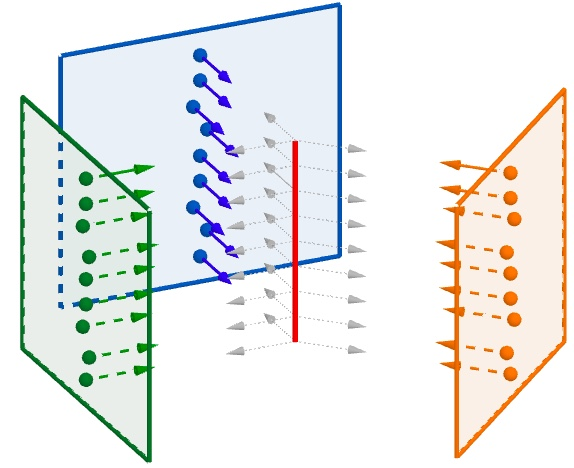
\includegraphics[scale=0.8]{10}
	\caption{Три множества точек, три плоскости и отрезок.}
	}
\end{figure}

\textbf{История задачи:}

Имеется отрезок и три плоскости. По трем заданным направлениям отрезок проецируется на эти плоскости, где мы получаем три отрезка.

Теперь стоит обратная задача. Даны три множества точек, каждое из которых находится на соответствующей плоскости. Направления изначального проецирования заданы. По этим наборам точек на плоскостях и по направлениям проецирования нужно найти исходный отрезок.

\newpage
\chapter{Решение}

\section{Метод №1}\label{meth1}

\subsection{Идея}\label{math1:idea}

\begin{itemize}
	\item[1)] Аппроксимируем множества точек прямыми.
	\item[2)] Проводим плоскости через полученные прямые и направления проектирования и получаем некую призму в пересечении трех плоскостей.
	\item[3)] Ищем прямую, минимально удаленную от данных трех плоскостей. 
\end{itemize}

\begin{center}
	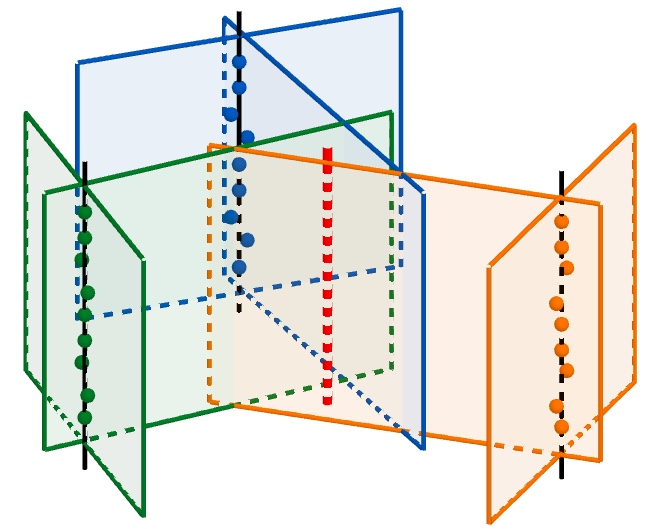
\includegraphics[scale=0.7]{11}

	Рис. 2.1: Построение прямых и плоскостей через точки множеств.
\end{center}

\subsection{Решение}\label{math1:solution}

Пусть имеем три множества:

\begin{center}
	$P_1 = \Set{p_i^1 = (x_i^1, y_i^1, z_i^1)}{i=\ton n_1}$

	\vspace{0.3cm}
	$P_2 = \Set{p_i^2 = (x_i^2, y_i^2, z_i^2)}{i=\ton n_2}$

	\vspace{0.3cm}
	$P_3 = \Set{p_i^3 = (x_i^3, y_i^3, z_i^3)}{i=\ton n_3}$
\end{center}

Используя алгоритм аппроксимации множества точек прямой \ref{line:alg:3dim}, получаем три прямые, приближающие наши множества $P_1$, $P_2$ и $P_3$:

\begin{center}
	$\mathit{l_1}: \; \begin{cases}
		x = x_0^1 + m^1 \cdot t \\
		y = y_0^1 + n^1 \cdot t \\
		z = z_0^1 + p^1 \cdot t
	\end{cases}$, где $t \in \mathbb{R}$ - параметр. 
\end{center}

\begin{center}
	$\mathit{l_2}: \; \begin{cases}
		x = x_0^2 + m^2 \cdot t \\
		y = y_0^2 + n^2 \cdot t \\
		z = z_0^2 + p^2 \cdot t
	\end{cases}$, где $t \in \mathbb{R}$ - параметр. 
\end{center}

\begin{center}
	$\mathit{l_3}: \; \begin{cases}
		x = x_0^3 + m^3 \cdot t \\
		y = y_0^3 + n^3 \cdot t \\
		z = z_0^3 + p^3 \cdot t
	\end{cases}$, где $t \in \mathbb{R}$ - параметр. 
\end{center}

Пусть $(m_1, n_1, p_1)^T$, $(m_2, n_2, p_2)^T$, $(m_3, n_3, p_3)^T$ - направления проектирования.

Тогда плоскости через найденные прямые и направления проектирования имеют вид:

\begin{center}
	$\mathit{\pi_1}: \; \begin{cases}
		x = x_0^1 + m^1 \cdot t_1 + m_1 \cdot t_2 \\
		y = y_0^1 + n^1 \cdot t_1 + n_1 \cdot t_2 \\
		z = z_0^1 + p^1 \cdot t_1 + p_1 \cdot t_2
	\end{cases}$, где $t_1, t_2 \in \mathbb{R}$ - параметры. 
\end{center}

\begin{center}
	$\mathit{\pi_2}: \; \begin{cases}
		x = x_0^2 + m^2 \cdot t_1 + m_2 \cdot t_2 \\
		y = y_0^2 + n^2 \cdot t_1 + n_2 \cdot t_2 \\
		z = z_0^2 + p^2 \cdot t_1 + p_2 \cdot t_2
	\end{cases}$, где $t_1, t_2 \in \mathbb{R}$ - параметры. 
\end{center}

\begin{center}
	$\mathit{\pi_3}: \; \begin{cases}
		x = x_0^3 + m^3 \cdot t_1 + m_3 \cdot t_2 \\
		y = y_0^3 + n^3 \cdot t_1 + n_3 \cdot t_2 \\
		z = z_0^3 + p^3 \cdot t_1 + p_3 \cdot t_2
	\end{cases}$, где $t_1, t_2 \in \mathbb{R}$ - параметры. 
\end{center}

Используя алгоритм нахождения прямой, минимально удаленной от данного множества плоскостей \ref{plane:alg:3dim}, получаем искомый отрезок (прямую).

\subsection{Погрешность и примеры работы программ}\label{math1:error}

Погрешность метода состоит из погрешности аппроксимации множеств точек прямыми и погрешности нахождения прямой, минимально удаленной от данного множества прямых.

\subsubsection{Искусственные данные}\label{math2:error:synth}

Исходные данные - три множетсва точек и три направления проектирования:

\begin{verbatim}
	(2, -4, 0)	          (-4, 2, 0)            (6.242641, 6.242641, 0)
	(2.1, -4, 1)         (-4, 2.1, 1)          (6.342641, 6.142641, 1)
	(1.9, -4, 2)         (-4, 1.9, 2)          (6.242641, 6.242641, 1.5)
	(2, -4, 3)           (-4, 2, 3)            (6.142641, 6.342641, 2)
	(2, -4, 4)           (-4, 2, 4)            (6.242641, 6.242641, 3)
	(2.1, -4, 5)         (-4, 2.1, 5)          (6.242641, 6.242641, 4)
	(1.9, -4, 6)         (-4, 1.9, 6)          (6.342641, 6.142641, 5)
	(2, -4, 7)           (-4, 2, 6.5)          (6.142641, 6.342641, 6)
	(2, -4, 7.5)         (-4, 2, 7)            (6.242641, 6.242641, 7)
	(2, -4, 8)           (-4, 2, 8)            (6.242641, 6.242641, 8)

	(0, 1, 0)            (1, 0, 0)             (-0.707107, -0.707107, 0)
\end{verbatim}

Полученные данные - направляющие векторы и точки прямых, аппроксимирующих исходные множества, а также две точки искомой прямой и значение функционала:

\begin{multicols}{2}
	\begin{verbatim}
		vector of line 1:
		(-0.002817, -0.000000, 1.000000)
		vector of line 2:
		(-0.000000, -0.003049, 1.000000)
		vector of line 3:
		(-0.003051, 0.003051, 1.000000)
	\end{verbatim}
	\columnbreak

	\begin{verbatim}
		point of line 1:
		(2.000001, -4.000001, 4.350000)
		point of line 2:
		(-4.000001, 2.000001, 4.250000)
		point of line 3:
		(6.242641, 6.242641, 3.750000)
\end{verbatim}
\end{multicols}
\begin{verbatim}
	TWO POINTS OF RESULT LINE:
	2.012064 2.000192 0.000000
	1.989034 2.000686 8.000000
	Lambda = 0.005286
\end{verbatim}

\begin{center}
	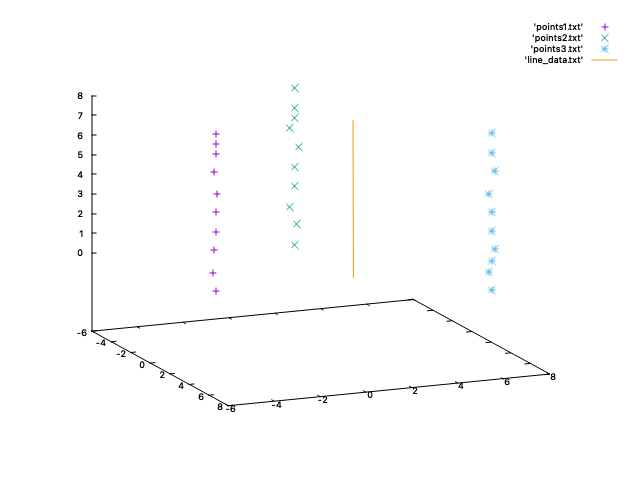
\includegraphics[scale=0.7]{meth1synth}
	\textit{полученный отрезок и исходные множества}
\end{center}

\begin{center}
	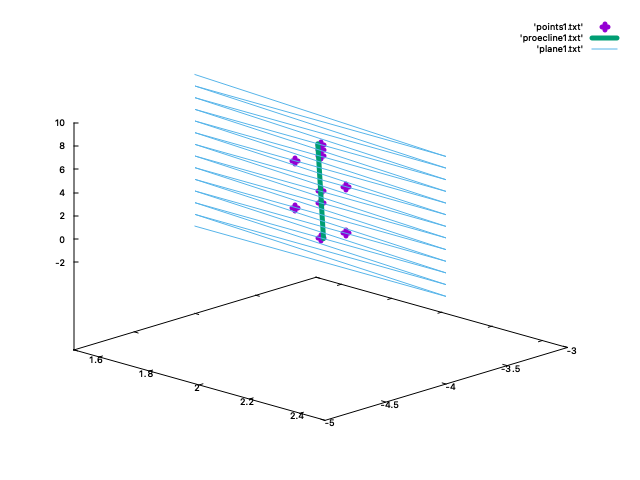
\includegraphics[scale=0.65]{meth1synthproec1}

	\textit{проекция полученного отрезка на плоскость первого множества}
	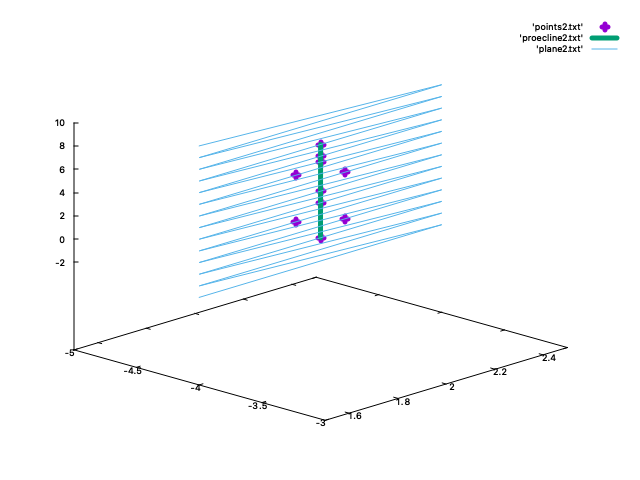
\includegraphics[scale=0.65]{meth1synthproec2}

	\textit{проекция полученного отрезка на плоскость второго множества}
	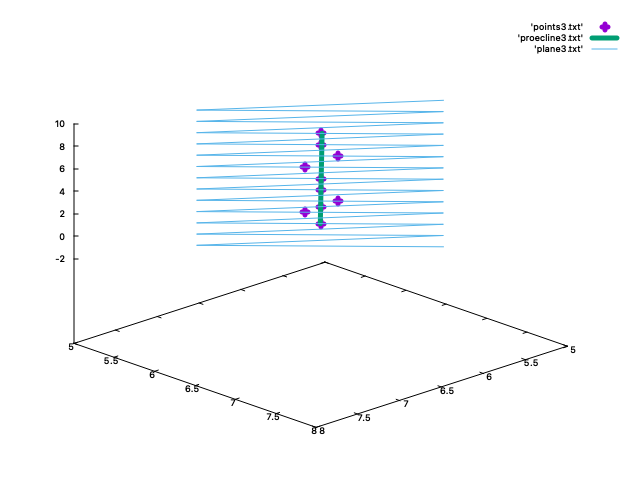
\includegraphics[scale=0.65]{meth1synthproec3}
	
	\textit{проекция полученного отрезка на плоскость третьего множества}
\end{center}

\subsubsection{Реальные данные}\label{math2:error:real}

Исходные данные - 100 множетсв точек и 100 направлений проектирования отрезка, ограниченного по $z$ значениями $-6.08332812434530$ и $-4.57712089734895$. Фигура симметричная, поэтому имеем два искомых отрезка.\\

Полученные данные - по две точки искомых прямых и значения функционала:

\begin{verbatim}
			DATA FOR POSITIVE SET:
	(3.227280, 2.584213, -6.083328)
	(2.505698, 1.505435, -4.577121)
	Lambda = 0.000003
			DATA FOR NEGATIVE SET:
	(-2.979147, -2.780110, -6.083328)
	(-2.377633, -1.727098, -4.577121)
	Lambda = 0.000030
\end{verbatim}

\begin{center}
	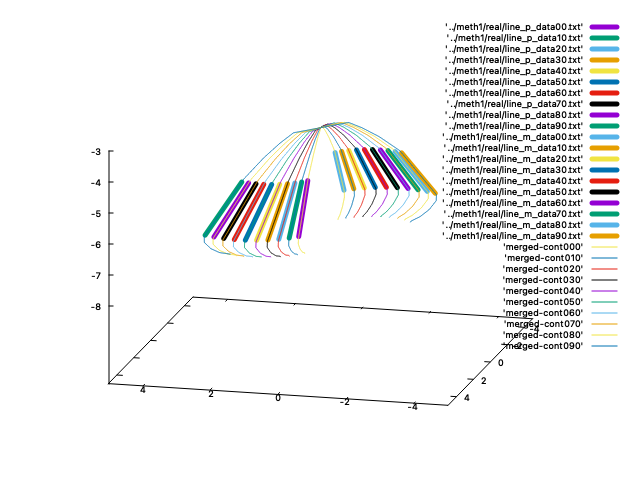
\includegraphics[scale=0.8]{meth1lineapprox}

	\textit{прямые, аппорксимирующие множества точек}

	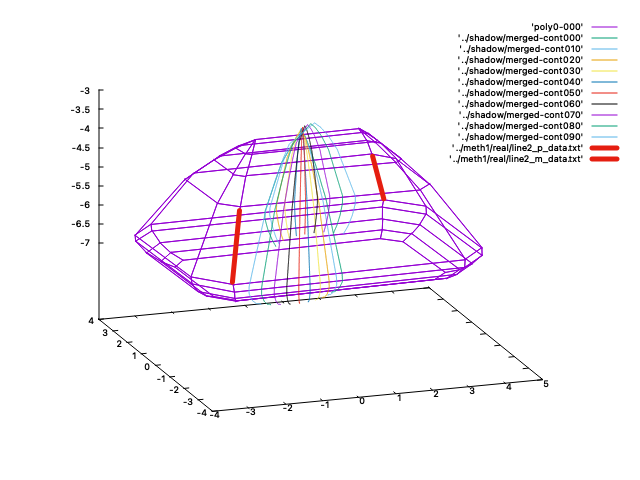
\includegraphics[scale=0.7]{meth1realresult}

	\textit{искомые отрезки, идеальный контур фигуры и исходные контуры проекций}

	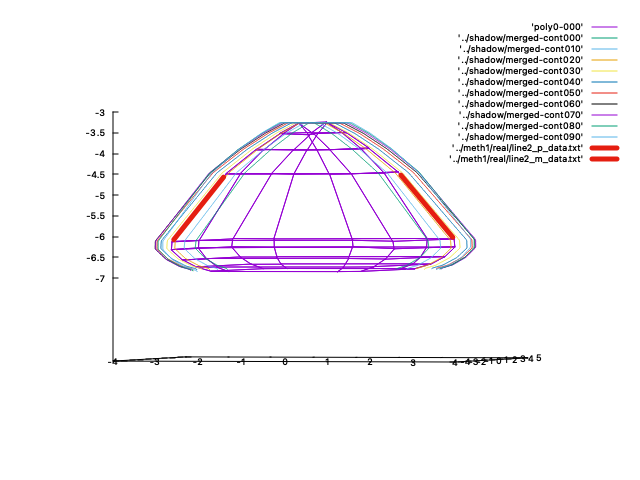
\includegraphics[scale=0.7]{meth1realsideview}

	\textit{искомые отрезки, идеальный контур фигуры и исходные контуры проекций}
\end{center}

\newpage
\section{Метод №2}\label{meth2}

\subsection{Идея}\label{math2:idea}

\begin{itemize}
	\item[1)] Выделяем сетку из всех значений координаты $z$ всех точек трех множеств.
	\item[2)] В каждом множестве добавляем точки с теми $z$, которые присутствуют в сетке, но отсутствуют в текущем множестве: эти точки добавляются на отрезки, соединяющие две ближашие точки множества. Таким образом, получаем разбиение точек трех множеств по "слоям".
	\item[3)] В каждом слое проводим прямые из точек, параллельные направлениям проектирования, и получаем некоторый треугольник. Находим точку, минимально удаленную от трех данных прямых.
	\item[4)] Аппроксимируем полученное множество точек прямой. 
\end{itemize}

\begin{center}
	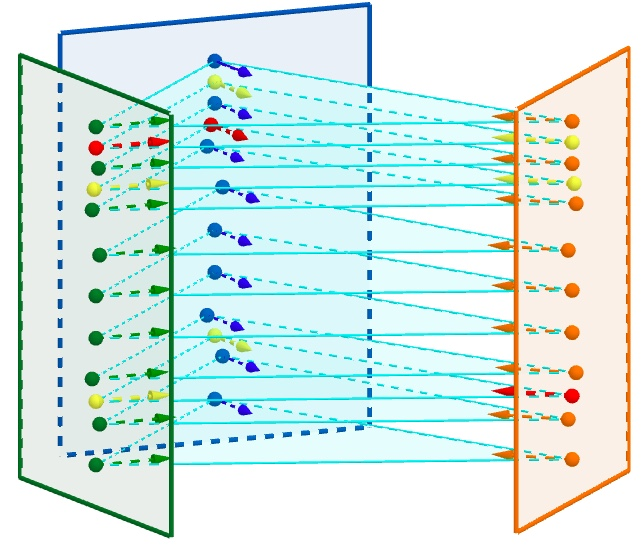
\includegraphics[scale=0.7]{120}

	Рис. 2.2: Добавление точек и разбивка по слоям.

	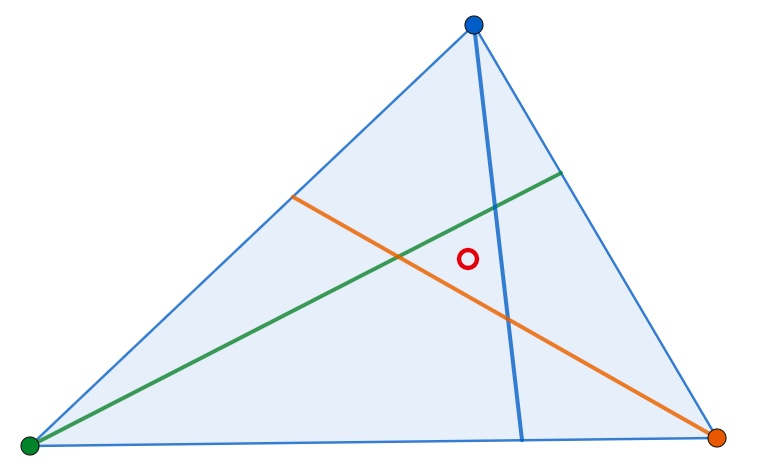
\includegraphics[scale=0.7]{122}

	Рис. 2.3: Нахождение точки, наименее удаленной от данных прямых.
\end{center}

\subsection{Решение}\label{math2:solution}

Алгоритм состоит в множественном применении алгоритма нахождении точки \ref{plane:alg:2dim} в каждом слое, минимально удаленных от проведенных прямых. После этого применяем алгоритм аппрокисимации множества полученных точек прямой \ref{line:alg:3dim}.

\subsection{Погрешность и примеры работы программ}\label{math2:error}

Погрешность складывается из погрешности добавления точек, погрешности множественного применения нахождения точек, минимально удаленных от прямых, и погрешности аппроксимации полученных точек прямой.\\

\newpage
\subsubsection{Искусственные данные}\label{math2:error:synth}

Исходные данные - три множетсва точек и три направления проектирования:

\begin{verbatim}
	(2, -4, 0)	          (-4, 2, 0)            (6.242641, 6.242641, 0)
	(2.1, -4, 1)         (-4, 2.1, 1)          (6.342641, 6.142641, 1)
	(1.9, -4, 2)         (-4, 1.9, 2)          (6.242641, 6.242641, 1.5)
	(2, -4, 3)           (-4, 2, 3)            (6.142641, 6.342641, 2)
	(2, -4, 4)           (-4, 2, 4)            (6.242641, 6.242641, 3)
	(2.1, -4, 5)         (-4, 2.1, 5)          (6.242641, 6.242641, 4)
	(1.9, -4, 6)         (-4, 1.9, 6)          (6.342641, 6.142641, 5)
	(2, -4, 7)           (-4, 2, 6.5)          (6.142641, 6.342641, 6)
	(2, -4, 7.5)         (-4, 2, 7)            (6.242641, 6.242641, 7)
	(2, -4, 8)           (-4, 2, 8)            (6.242641, 6.242641, 8)

	(0, 1, 0)            (1, 0, 0)             (-0.707107, -0.707107, 0)
\end{verbatim}

Полученные данные - направляющий вектор прямой, точка прямой и значение функционала:

\begin{verbatim}
	l = (-0.004403, -0.001467, 1.000000)
	p = (1.999266, 2.000773, 4.291667)
	Lambda = 0.006596
\end{verbatim}

\begin{center}
	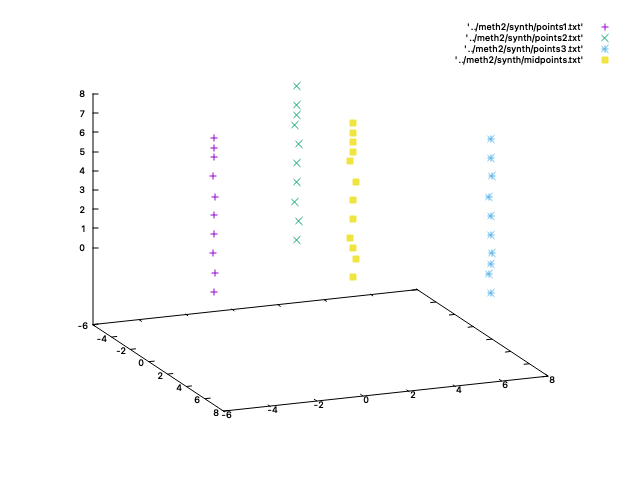
\includegraphics[scale=0.65]{meth2synthmidpoints}

	\textit{<<средние>> точки в каждом слое и исходные множества}

	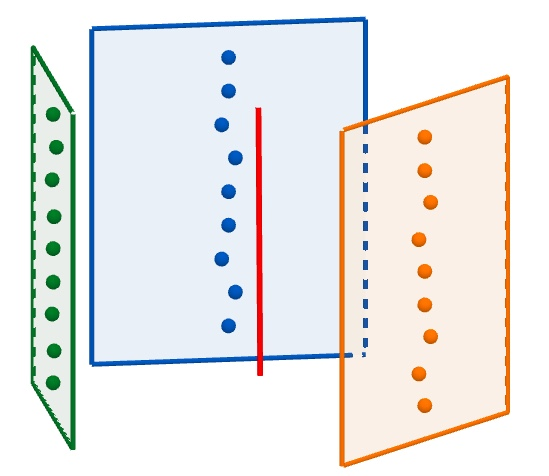
\includegraphics[scale=0.7]{meth2synth}

	\textit{полученный отрезок и исходные множества}
\end{center}

\subsubsection{Реальные данные}\label{math2:error:real}

Исходные данные - 100 множетсв точек и 100 направлений проектирования отрезка, ограниченного по $z$ значениями $-6.08332812434530$ и $-4.57712089734895$. Фигура симметричная, поэтому имеем два искомых отрезка.\\

Полученные данные - по две точки искомых прямых и значения функционала:

\begin{verbatim}
			DATA FOR POSITIVE SET:
	(3.227402, 2.584165, -6.083328)
	(2.505786, 1.505411, -4.577121)
	Lambda = 0.007525
			DATA FOR NEGATIVE SET:
	(-2.979351, -2.779962, -6.083328)
	(-2.377752, -1.727015, -4.577121)
	Lambda = 0.000030
\end{verbatim}

\begin{center}
	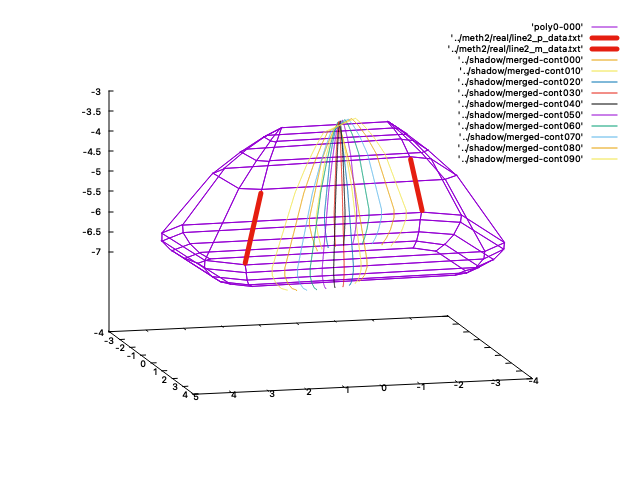
\includegraphics[scale=0.7]{meth2real}

	\textit{искомые отрезки, идеальный контур фигуры и исходные контуры проекций}

	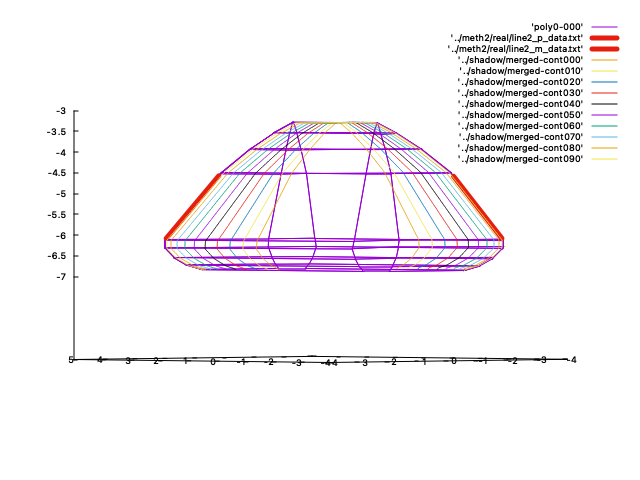
\includegraphics[scale=0.7]{meth2realsideview}

	\textit{искомые отрезки, идеальный контур фигуры и исходные контуры проекций}
\end{center}

\newpage
% \section{Метод №3}\label{meth3}

\subsection{Идея}\label{math3:idea}

\begin{itemize}
	\item[1)] Проводим прямые через точки множеств в направлениях проектирования и получаем множество скрещивающихся прямых.
	\item[2)] Рассматривая искомую прямую как вектор, приложенный к точке, фиксируем точку и составляем функционал суммы квадратов расстояний от проекций прямой до соответствующих множеств точек и минимизируем его (получаем линейную систему).
	\item[3)] Аналогично рассматривая искомую прямую как вектор, приложенный к точке, теперь фиксируем вектор и составляем функционал суммы квадратов расстояний от проекций прямой до соответствующих множеств точек и минимизируем его (тоже получаем линейную систему).
	\item[4)] Некоторыми последовательными изменениями одного параметра при фиксированном другом и наоборот (вектор и точка), минимизируем полученные функционалы и минимизируем отклонение.
\end{itemize}

\begin{center}
	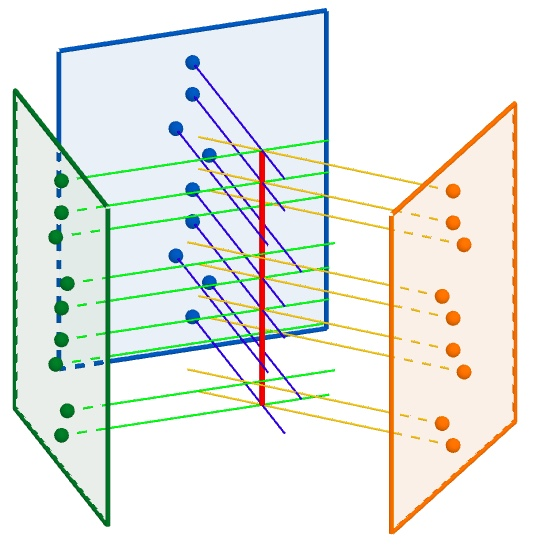
\includegraphics[scale=0.6]{131}

	Рис. 2.4: Построение скрещивающихся прямых через точки множеств.
\end{center}

\begin{center}
	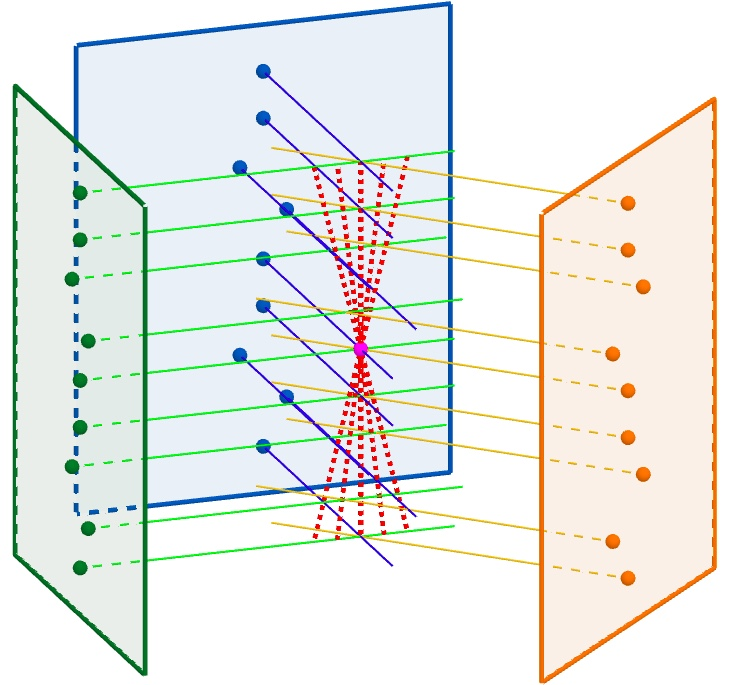
\includegraphics[scale=0.48]{132}

	Рис. 2.5: Изменение вектора прямой при фиксированной точке.

	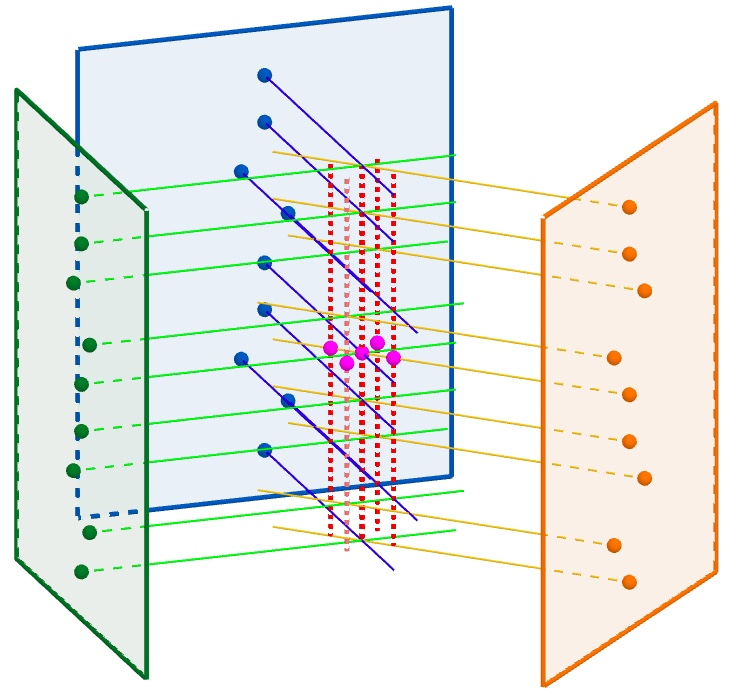
\includegraphics[scale=0.48]{133}

	Рис. 2.6: Изменение точки прямой при фиксированном векторе.
\end{center}

\subsection{Решение}\label{math3:solution}

Пусть имеем три множества:

\begin{center}
	$P_1 = \Set{p_i^1 = (x_i^1, y_i^1, z_i^1)}{i=\ton n_1}$

	\vspace{0.3cm}
	$P_2 = \Set{p_i^2 = (x_i^2, y_i^2, z_i^2)}{i=\ton n_2}$

	\vspace{0.3cm}
	$P_3 = \Set{p_i^3 = (x_i^3, y_i^3, z_i^3)}{i=\ton n_3}$
\end{center}

Также имеем три направления проектирования (векторы нормали плоскостей, которым принадлежат множества $P_1, P_2$ и $P_3$):
$$\begin{gathered}
	r_1 = (r_1^1, r_2^1, r_3^1) \\
	r_2 = (r_1^2, r_2^2, r_3^2) \\
	r_3 = (r_1^3, r_2^3, r_3^3)
\end{gathered}$$

Будем искать прямую в параметрическом виде. Пусть $(m, n, p)$ - напрявляющий вектор прямой, $(x_0, y_0, z_0)$ - некоторая точка прямой. Тогда следующая система задает прямую в $\mathbb{R}^3$: 

\begin{center}
	$\mathit{l}: \; \begin{cases}
		x = x_0 + m \cdot t \\
		y = y_0 + n \cdot t \\
		z = z_0 + p \cdot t
	\end{cases}$, где $t \in \mathbb{R}$ - параметр. 
\end{center}

Проведем через нашу прямую и направления проектирования плоскости:

\begin{center}
	$\pi_1: \; \begin{cases}
		x = x_0 + m \cdot t_1 + r_1^1 \cdot t_2 \\
		y = y_0 + n \cdot t_1 + r_2^1 \cdot t_2 \\
		z = z_0 + p \cdot t_1 + r_3^1 \cdot t_2
	\end{cases}$, где $t_1, t_2 \in \mathbb{R}$ - параметры. 

	\vspace{0.2cm}
	$\pi_2: \; \begin{cases}
		x = x_0 + m \cdot t_1 + r_1^2 \cdot t_2 \\
		y = y_0 + n \cdot t_1 + r_2^2 \cdot t_2 \\
		z = z_0 + p \cdot t_1 + r_3^2 \cdot t_2
	\end{cases}$, где $t_1, t_2 \in \mathbb{R}$ - параметры. 

	\vspace{0.2cm}
	$\pi_3: \; \begin{cases}
		x = x_0 + m \cdot t_1 + r_1^3 \cdot t_2 \\
		y = y_0 + n \cdot t_1 + r_2^3 \cdot t_2 \\
		z = z_0 + p \cdot t_1 + r_3^3 \cdot t_2
	\end{cases}$, где $t_1, t_2 \in \mathbb{R}$ - параметры. 
\end{center}
\newpage
Чтобы найти общие уравнения этих плоскостей, найдем нормали этих плоскостей, которые будем искать как векторное произведение напрявляющих векторов:

$$\begin{gathered}
	n_1 = [l, r_1] = \begin{vmatrix}
		i & j & k \\
		m & n & p \\
		r_1^1 & r_2^1 & r_3^1
	\end{vmatrix} = \left( \begin{vmatrix}
		n & p \\
		r_2^1 & r_3^1
	\end{vmatrix}, -\begin{vmatrix}
		m & p \\
		r_1^1 & r_3^1
	\end{vmatrix}, \begin{vmatrix}
		m & n \\
		r_1^1 & r_2^1
	\end{vmatrix} \right) = \\
	= \left( n r_3^1 - p r_2^1, p r_1^1 - m r_3^1, m r_2^1 - n r_1^1 \right)
\end{gathered}$$
$$\begin{gathered}
	n_2 = [l, r_2] = \begin{vmatrix}
		i & j & k \\
		m & n & p \\
		r_1^2 & r_2^2 & r_3^2
	\end{vmatrix} = \left( \begin{vmatrix}
		n & p \\
		r_2^2 & r_3^2
	\end{vmatrix}, -\begin{vmatrix}
		m & p \\
		r_1^2 & r_3^2
	\end{vmatrix}, \begin{vmatrix}
		m & n \\
		r_1^2 & r_2^2
	\end{vmatrix} \right) = \\
	= \left( n r_3^2 - p r_2^2, p r_1^2 - m r_3^2, m r_2^2 - n r_1^2 \right)
\end{gathered}$$
$$\begin{gathered}
	n_3 = [l, r_3] = \begin{vmatrix}
		i & j & k \\
		m & n & p \\
		r_1^3 & r_2^3 & r_3^3
	\end{vmatrix} = \left( \begin{vmatrix}
		n & p \\
		r_2^3 & r_3^3
	\end{vmatrix}, -\begin{vmatrix}
		m & p \\
		r_1^3 & r_3^3
	\end{vmatrix}, \begin{vmatrix}
		m & n \\
		r_1^3 & r_2^3
	\end{vmatrix} \right) = \\
	= \left( n r_3^3 - p r_2^3, p r_1^3 - m r_3^3, m r_2^3 - n r_1^3 \right)
\end{gathered}$$

Отнормируем векторы нормалей:
$$\begin{gathered}
	(A_1, B_1, C_1) = \frac{\left( n r_3^1 - p r_2^1, p r_1^1 - m r_3^1, m r_2^1 - n r_1^1 \right)}{\sqrt{(n r_3^1 - p r_2^1)^2 + (p r_1^1 - m r_3^1)^2 + (m r_2^1 - n r_1^1)^2}} \\
	(A_2, B_2, C_2) = \frac{\left( n r_3^2 - p r_2^2, p r_1^2 - m r_3^2, m r_2^2 - n r_1^2 \right)}{\sqrt{(n r_3^2 - p r_2^2)^2 + (p r_1^2 - m r_3^2)^2 + (m r_2^2 - n r_1^2)^2}} \\
	(A_3, B_3, C_3) = \frac{\left( n r_3^3 - p r_2^3, p r_1^3 - m r_3^3, m r_2^3 - n r_1^3 \right)}{\sqrt{(n r_3^3 - p r_2^3)^2 + (p r_1^3 - m r_3^3)^2 + (m r_2^3 - n r_1^3)^2}}
\end{gathered}$$

Тогда общие уравнения плоскостей имеют вид:
$$\begin{gathered}
	\pi_1: \; A_1 (x - x_0) + B_1 (y - y_0) + C_1 (z - z_0) = 0 \\
	\pi_2: \; A_2 (x - x_0) + B_2 (y - y_0) + C_2 (z - z_0) = 0 \\
	\pi_3: \; A_3 (x - x_0) + B_3 (y - y_0) + C_3 (z - z_0) = 0 
\end{gathered}$$
Иначе:
$$\begin{gathered}
	\pi_1: \; A_1 x + B_1 y + C_1 z + D_1 = 0 \\
	\pi_2: \; A_2 x + B_2 y + C_2 z + D_2 = 0 \\
	\pi_3: \; A_3 x + B_3 y + C_3 z + D_3 = 0
\end{gathered}$$
$$\begin{gathered}
	\begin{cases}
		A_1 = \frac{n r_3^1 - p r_2^1}{\sqrt{(n r_3^1 - p r_2^1)^2 + (p r_1^1 - m r_3^1)^2 + (m r_2^1 - n r_1^1)^2}} \\
		B_1 = \frac{p r_1^1 - m r_3^1}{\sqrt{(n r_3^1 - p r_2^1)^2 + (p r_1^1 - m r_3^1)^2 + (m r_2^1 - n r_1^1)^2}} \\
		C_1 = \frac{m r_2^1 - n r_1^1}{\sqrt{(n r_3^1 - p r_2^1)^2 + (p r_1^1 - m r_3^1)^2 + (m r_2^1 - n r_1^1)^2}} \\
		D_1 = \frac{- (n r_3^1 - p r_2^1) x_0 - (p r_1^1 - m r_3^1) y_0 - (m r_2^1 - n r_1^1) z_0}{\sqrt{(n r_3^1 - p r_2^1)^2 + (p r_1^1 - m r_3^1)^2 + (m r_2^1 - n r_1^1)^2}}
	\end{cases} \\
	\begin{cases}
		A_2 = \frac{n r_3^2 - p r_2^2}{\sqrt{(n r_3^2 - p r_2^2)^2 + (p r_1^2 - m r_3^2)^2 + (m r_2^2 - n r_1^2)^2}} \\
		B_2 = \frac{p r_1^2 - m r_3^2}{\sqrt{(n r_3^2 - p r_2^2)^2 + (p r_1^2 - m r_3^2)^2 + (m r_2^2 - n r_1^2)^2}} \\
		C_2 = \frac{m r_2^2 - n r_1^2}{\sqrt{(n r_3^2 - p r_2^2)^2 + (p r_1^2 - m r_3^2)^2 + (m r_2^2 - n r_1^2)^2}} \\
		D_2 = \frac{- (n r_3^2 - p r_2^2) x_0 - (p r_1^2 - m r_3^2) y_0 - (m r_2^2 - n r_1^2) z_0}{\sqrt{(n r_3^2 - p r_2^2)^2 + (p r_1^2 - m r_3^2)^2 + (m r_2^2 - n r_1^2)^2}}
	\end{cases} \\
	\begin{cases}
		A_3 = \frac{n r_3^3 - p r_2^3}{\sqrt{(n r_3^3 - p r_2^3)^2 + (p r_1^3 - m r_3^3)^2 + (m r_2^3 - n r_1^3)^2}} \\
		B_3 = \frac{p r_1^3 - m r_3^3}{\sqrt{(n r_3^3 - p r_2^3)^2 + (p r_1^3 - m r_3^3)^2 + (m r_2^3 - n r_1^3)^2}} \\
		C_3 = \frac{m r_2^3 - n r_1^3}{\sqrt{(n r_3^3 - p r_2^3)^2 + (p r_1^3 - m r_3^3)^2 + (m r_2^3 - n r_1^3)^2}} \\
		D_3 = \frac{- (n r_3^3 - p r_2^3) x_0 - (p r_1^3 - m r_3^3) y_0 - (m r_2^3 - n r_1^3) z_0}{\sqrt{(n r_3^3 - p r_2^3)^2 + (p r_1^3 - m r_3^3)^2 + (m r_2^3 - n r_1^3)^2}}
	\end{cases}
\end{gathered}$$

Найдем плоскости, которым принадлежат множества точек:
$$\begin{gathered}
	w_1: \; r_1^1 x + r_2^1 y + r_3^1 z - (r_1^1 x_1^1 + r_2^1 y_1^1 + r_3^1 z_1^1) = 0 \\
	w_2: \; r_1^2 x + r_2^2 y + r_3^2 z - (r_1^2 x_1^2 + r_2^2 y_1^2 + r_3^2 z_1^2) = 0 \\
	w_3: \; r_1^3 x + r_2^3 y + r_3^3 z - (r_1^3 x_1^3 + r_2^3 y_1^3 + r_3^3 z_1^3) = 0
\end{gathered}$$

В пересечении плоскостей $\pi_1$ и $w_1$, $\pi_2$ и $w_2$, $\pi_3$ и $w_3$ получаем проекции исходного отрезка $l_1, l_2, l_3$ на плоскости множеств $w_1, w_2, w_3$. Тогда расстояния от точек множества $P_i$ до проекции $l_i$ на соответствующую плоскость $w_i$ равно расстоянию от этих точек до плоскости $\pi_i$, проходящую через искомый отрезок $l$.

$$\rho (p_i^j, l_j) = |A_j x_i^j + B_j y_i^j + C_j z_i^j + D_j|$$
где $i$ - номер соответствующей точки множества,

$j$ - номер соответствующей плоскости $\pi_j$.\\

Тогда функционал суммы квадратов расстояний от точек множеств до проекций исходного отрезка равен:
$$\Lambda = \underset{j=1}{\overset{3}{\sum}}\underset{i=1}{\overset{n_1, n_2, n_3}{\sum}}(A_j x_i^j + B_j y_i^j + C_j z_i^j + D_j)^2$$
\newpage
Рассмотрим параллельный сдвиг исходного отрезка на некоторый вектор $h$. Будем рассматривать вектор $h$ как вектор, лежащий в плоскости, параллельной OXY, тогда $h = (x_h, y_h, 0)$ и сдвиг будет харакетризоваться этим вектором $h$ полнсотью.\\

Более того, при параллельном переносе исходного отрезка плоскости $\pi_i$ также переносятся параллельно себе, т.е. векторы нормали не изменятся, а изменятся лишь коэффициенты $D_i$ - они умножатся на скалярное произведение вектора $h$ и вектора нормали плоскости $(A_i, B_i, C_i)$. Таким образом, уравнение новых плоскостей $\pi'_j$ будет иметь вид:
$$\begin{gathered}
	A_j x + B_j y + C_j z + D_j \left(h, (A_j, B_j, C_j) \right) = 0 \; \Rightarrow \\
	\Rightarrow \; A_j x + B_j y + C_j z + D_j (x_h A_j + y_h B_j) = 0
\end{gathered}$$

Тогда соответствующий функционал после сдвига имеет вид:
$$\Lambda = \underset{j=1}{\overset{3}{\sum}}\underset{i=1}{\overset{n_1, n_2, n_3}{\sum}}\left(A_j x_i^j + B_j y_i^j + C_j z_i^j + D_j(x_h A_j + y_h B_j)\right)^2$$

Найдем частные производные функционала по $x_h$ и $y_h$:
$$\begin{gathered}
	\begin{cases}
		\frac{\partial}{\partial x_h} \underset{j=1}{\overset{3}{\sum}}\underset{i=1}{\overset{n_1, n_2, n_3}{\sum}}\left(A_j x_i^j + B_j y_i^j + C_j z_i^j + D_j(x_h A_j + y_h B_j)\right)^2 = 0 \\
		\frac{\partial}{\partial y_h} \underset{j=1}{\overset{3}{\sum}}\underset{i=1}{\overset{n_1, n_2, n_3}{\sum}}\left(A_j x_i^j + B_j y_i^j + C_j z_i^j + D_j(x_h A_j + y_h B_j)\right)^2 = 0
	\end{cases} \\
	\begin{cases}
		 \underset{j=1}{\overset{3}{\sum}}\underset{i=1}{\overset{n_1, n_2, n_3}{\sum}}\frac{\partial}{\partial x_h}\left(A_j x_i^j + B_j y_i^j + C_j z_i^j + D_j(x_h A_j + y_h B_j)\right)^2 = 0 \\
		 \underset{j=1}{\overset{3}{\sum}}\underset{i=1}{\overset{n_1, n_2, n_3}{\sum}}\frac{\partial}{\partial y_h}\left(A_j x_i^j + B_j y_i^j + C_j z_i^j + D_j(x_h A_j + y_h B_j)\right)^2 = 0
	\end{cases}\\
	\begin{cases}
		 \underset{j=1}{\overset{3}{\sum}}\underset{i=1}{\overset{n_1, n_2, n_3}{\sum}}\Bigg(2 \left(A_j x_i^j + B_j y_i^j + C_j z_i^j + D_j(x_h A_j + y_h B_j)\right) A_j D_j\Bigg) = 0 \\
		 \underset{j=1}{\overset{3}{\sum}}\underset{i=1}{\overset{n_1, n_2, n_3}{\sum}}\Bigg(2 \left(A_j x_i^j + B_j y_i^j + C_j z_i^j + D_j(x_h A_j + y_h B_j)\right) B_j D_j\Bigg) = 0
	\end{cases}\\
	\begin{cases}
		\underset{j=1}{\overset{3}{\sum}}\underset{i=1}{\overset{n_1, n_2, n_3}{\sum}}\Bigg( A_j^2 D_j^2 x_h + A_j B_j D_j^2 y_h + A_j D_j \left(  A_j x_i^j + B_j y_i^j + C_j z_i^j\right) \Bigg) = 0 \\
		\underset{j=1}{\overset{3}{\sum}}\underset{i=1}{\overset{n_1, n_2, n_3}{\sum}}\Bigg( A_j B_j D_j^2 x_h + B_j^2 D_j^2 y_h + B_j D_j \left( A_j x_i^j + B_j y_i^j + C_j z_i^j \right) \Bigg) = 0
	\end{cases}
\end{gathered}$$
\newpage
Получаем линейную систему на $x_h, y_h$:
$$\begin{cases}
	\Bigg( \underset{j=1}{\overset{3}{\sum}}\underset{i=1}{\overset{n_1, n_2, n_3}{\sum}} A_j^2 D_j^2 \Bigg) x_h + \Bigg( \underset{j=1}{\overset{3}{\sum}}\underset{i=1}{\overset{n_1, n_2, n_3}{\sum}} A_j B_j D_j^2 \Bigg) y_h + \\
	\hspace{1cm} + \Bigg( \underset{j=1}{\overset{3}{\sum}}\underset{i=1}{\overset{n_1, n_2, n_3}{\sum}} A_j D_j \left(  A_j x_i^j + B_j y_i^j + C_j z_i^j\right) \Bigg) = 0 \\
	\Bigg( \underset{j=1}{\overset{3}{\sum}}\underset{i=1}{\overset{n_1, n_2, n_3}{\sum}} A_j B_j D_j^2 \Bigg) x_h + \Bigg( \underset{j=1}{\overset{3}{\sum}}\underset{i=1}{\overset{n_1, n_2, n_3}{\sum}} B_j^2 D_j^2 \Bigg) y_h + \\
	\hspace{1cm} + \Bigg( \underset{j=1}{\overset{3}{\sum}}\underset{i=1}{\overset{n_1, n_2, n_3}{\sum}} B_j D_j \left( A_j x_i^j + B_j y_i^j + C_j z_i^j \right) \Bigg) = 0
\end{cases}$$
Введем обозначения:
$$\begin{cases}
	a_{11} = \underset{j=1}{\overset{3}{\sum}}\underset{i=1}{\overset{n_1, n_2, n_3}{\sum}} A_j^2 D_j^2 \\
	a_{12} = a_{21} = \underset{j=1}{\overset{3}{\sum}}\underset{i=1}{\overset{n_1, n_2, n_3}{\sum}} A_j B_j D_j^2 \\
	a_{22} = \underset{j=1}{\overset{3}{\sum}}\underset{i=1}{\overset{n_1, n_2, n_3}{\sum}} B_j^2 D_j^2 \\
	b_1 = \underset{j=1}{\overset{3}{\sum}}\underset{i=1}{\overset{n_1, n_2, n_3}{\sum}} A_j D_j \left(  A_j x_i^j + B_j y_i^j + C_j z_i^j\right) \\
	b_2 = \underset{j=1}{\overset{3}{\sum}}\underset{i=1}{\overset{n_1, n_2, n_3}{\sum}} B_j D_j \left( A_j x_i^j + B_j y_i^j + C_j z_i^j \right)
\end{cases}$$
Если система невырождена, то получаем решение:
$$\begin{cases}
	x_h = \frac{a_{22} b_1 - a_{12} b_2}{a_{12}^2 - a_{11}a_{22}} \\
	y_h = \frac{a_{11} b_2 - a_{12} b_1}{a_{12}^2 - a_{11}a_{22}}
\end{cases}$$

\vspace{0.5cm}
Теперь будем рассматривать поворот исходного отрезка вокруг точки $(x_0, y_0, z_0)$ - середины отрезка. Пусть один конец переместили на вектор $h = (x_h, y_h, 0)$, тогда новое уравнение прямой имеет вид:

\begin{center}
	$\mathit{l}: \; \begin{cases}
		x = x_0 + (m + x_h) \cdot t \\
		y = y_0 + (n + y_h) \cdot t \\
		z = z_0 + p \cdot t
	\end{cases}$, где $t \in \mathbb{R}$ - параметр. 
\end{center}

Тогда уравнения плоскостей, проходящие через повернутую прямую имеют вид:
$$\begin{gathered}
	\pi_1: \; A_1 x + B_1 y + C_1 z + D_1 = 0 \\
	\pi_2: \; A_2 x + B_2 y + C_2 z + D_2 = 0 \\
	\pi_3: \; A_3 x + B_3 y + C_3 z + D_3 = 0
\end{gathered}$$
$$\begin{gathered}
	\begin{cases}
		A_1 = \frac{(n + y_h) r_3^1 - p r_2^1}{\sqrt{((n + y_h) r_3^1 - p r_2^1)^2 + (p r_1^1 - (m + x_h) r_3^1)^2 + ((m + x_h) r_2^1 - (n + y_h) r_1^1)^2}} \\
		B_1 = \frac{p r_1^1 - (m + x_h) r_3^1}{\sqrt{((n + y_h) r_3^1 - p r_2^1)^2 + (p r_1^1 - (m + x_h) r_3^1)^2 + ((m + x_h) r_2^1 - (n + y_h) r_1^1)^2}} \\
		C_1 = \frac{(m + x_h) r_2^1 - (n + y_h) r_1^1}{\sqrt{((n + y_h) r_3^1 - p r_2^1)^2 + (p r_1^1 - (m + x_h) r_3^1)^2 + ((m + x_h) r_2^1 - (n + y_h) r_1^1)^2}} \\
		D_1 = \frac{- ((n + y_h) r_3^1 - p r_2^1) x_0 - (p r_1^1 - (m + x_h) r_3^1) y_0 - ((m + x_h) r_2^1 - (n + y_h) r_1^1) z_0}{\sqrt{((n + y_h) r_3^1 - p r_2^1)^2 + (p r_1^1 - (m + x_h) r_3^1)^2 + ((m + x_h) r_2^1 - (n + y_h) r_1^1)^2}}
	\end{cases} \\
	\begin{cases}
		A_2 = \frac{(n + y_h) r_3^2 - p r_2^2}{\sqrt{((n + y_h) r_3^2 - p r_2^2)^2 + (p r_1^2 - (m + x_h) r_3^2)^2 + ((m + x_h) r_2^2 - (n + y_h) r_1^2)^2}} \\
		B_2 = \frac{p r_1^2 - (m + x_h) r_3^2}{\sqrt{((n + y_h) r_3^2 - p r_2^2)^2 + (p r_1^2 - (m + x_h) r_3^2)^2 + ((m + x_h) r_2^2 - (n + y_h) r_1^2)^2}} \\
		C_2 = \frac{(m + x_h) r_2^2 - (n + y_h) r_1^2}{\sqrt{((n + y_h) r_3^2 - p r_2^2)^2 + (p r_1^2 - (m + x_h) r_3^2)^2 + ((m + x_h) r_2^2 - (n + y_h) r_1^2)^2}} \\
		D_2 = \frac{- ((n + y_h) r_3^2 - p r_2^2) x_0 - (p r_1^2 - (m + x_h) r_3^2) y_0 - ((m + x_h) r_2^2 - (n + y_h) r_1^2) z_0}{\sqrt{((n + y_h) r_3^2 - p r_2^2)^2 + (p r_1^2 - (m + x_h) r_3^2)^2 + ((m + x_h) r_2^2 - (n + y_h) r_1^2)^2}}
	\end{cases} \\
	\begin{cases}
		A_3 = \frac{(n + y_h) r_3^3 - p r_2^3}{\sqrt{((n + y_h) r_3^3 - p r_2^3)^2 + (p r_1^3 - (m + x_h) r_3^3)^2 + ((m + x_h) r_2^3 - (n + y_h) r_1^3)^2}} \\
		B_3 = \frac{p r_1^3 - (m + x_h) r_3^3}{\sqrt{((n + y_h) r_3^3 - p r_2^3)^2 + (p r_1^3 - (m + x_h) r_3^3)^2 + ((m + x_h) r_2^3 - (n + y_h) r_1^3)^2}} \\
		C_3 = \frac{(m + x_h) r_2^3 - (n + y_h) r_1^3}{\sqrt{((n + y_h) r_3^3 - p r_2^3)^2 + (p r_1^3 - (m + x_h) r_3^3)^2 + ((m + x_h) r_2^3 - (n + y_h) r_1^3)^2}} \\
		D_3 = \frac{- ((n + y_h) r_3^3 - p r_2^3) x_0 - (p r_1^3 - (m + x_h) r_3^3) y_0 - ((m + x_h) r_2^3 - (n + y_h) r_1^3) z_0}{\sqrt{((n + y_h) r_3^3 - p r_2^3)^2 + (p r_1^3 - (m + x_h) r_3^3)^2 + ((m + x_h) r_2^3 - (n + y_h) r_1^3)^2}}
	\end{cases}
\end{gathered}$$

\vspace{1cm}
Вместо выражения исходного функционала суммы квадратов расстояний рассмотрим лишь числитель функционала, получаем следующий функционал для каждого из множеств:
$$\begin{gathered}
	\Lambda' = \underset{i=1}{\overset{n_j}{\sum}} \Bigg( \left( (n+y_h)r_3^j - p r_2^j \right)x_i^j + \left( p r_1^j - (m+x_h) r_3^j \right)y_i^j + \\ 
	\hspace{0.5cm} + \left( (m+x_h)r_2^j - (n+y_h)r_1^j \right) z_i^j - ((n + y_h) r_3^j - p r_2^j) x_0 -  \\
	\hspace{1cm} - (p r_1^j - (m + x_h) r_3^j) y_0 - ((m + x_h) r_2^j - (n + y_h) r_1^j) z_0 \Bigg)^2 \\
	j = 1,2,3
\end{gathered}$$

Мы не можем суммировать все суммы квадратов, т.к. для разных плоскостей разные выражения в знаменателе, и избавиться от всех них при подсчете не получится.\\

Чтобы получить единственный оптимальный поворот для всех плоскостей решим проблему знаменателей следующим образом. При итерации поворота в знаменатели подставим значения $x_h$ и $y_h$ предыдущей итерации, на начальном шаге возьмем нулевые $x_h$ и $y_h$. Таким образом мы будем рассматривать сумму значений функционалов для плоскостей с некоторыми весами, равными обратным значениям знаменателей с подставновкой, описанной выше. Эту сумму и необходимо будет минимизировать по $x_h$ и $y_h$. Новый функционал имеет вид:
$$\begin{gathered}
	\Lambda' = \underset{i=1}{\overset{3}{\sum}}w_{i-1}\underset{j=1}{\overset{n_i}{\sum}} \Bigg( \left( (n+y_h)r_3^j - p r_2^j \right)x_i^j + \left( p r_1^j - (m+x_h) r_3^j \right)y_i^j + \\ 
	\hspace{0.5cm} + \left( (m+x_h)r_2^j - (n+y_h)r_1^j \right) z_i^j - ((n + y_h) r_3^j - p r_2^j) x_0 -  \\
	\hspace{1cm} - (p r_1^j - (m + x_h) r_3^j) y_0 - ((m + x_h) r_2^j - (n + y_h) r_1^j) z_0 \Bigg)^2 \\
	j = 1,2,3, \;\; w_{i-1} \text{ - значение знаменателя при } x_h, y_h \text{ из предыдущей итерации}
\end{gathered}$$
Найдем частные производные функционала по $x_h$ и $y_h$:
$$\begin{gathered}
	\begin{cases}
		\frac{\partial}{\partial x_h} \underset{i=1}{\overset{3}{\sum}}w_{i-1}\underset{j=1}{\overset{n_i}{\sum}} \Bigg( \left( (n+y_h)r_3^j - p r_2^j \right)x_i^j + \left( p r_1^j - (m+x_h) r_3^j \right)y_i^j + \\
		\hspace{1.5cm} + \left( (m+x_h)r_2^j - (n+y_h)r_1^j \right) z_i^j - ((n + y_h) r_3^j - p r_2^j) x_0 - \\
		\hspace{1.5cm} - (p r_1^j - (m + x_h) r_3^j) y_0 - ((m + x_h) r_2^j - (n + y_h) r_1^j) z_0 \Bigg)^2 = 0 \\
		\frac{\partial}{\partial y_h} \underset{i=1}{\overset{3}{\sum}}w_{i-1}\underset{j=1}{\overset{n_i}{\sum}} \Bigg( \left( (n+y_h)r_3^j - p r_2^j \right)x_i^j + \left( p r_1^j - (m+x_h) r_3^j \right)y_i^j + \\
		\hspace{1.5cm} + \left( (m+x_h)r_2^j - (n+y_h)r_1^j \right) z_i^j - ((n + y_h) r_3^j - p r_2^j) x_0 - \\
		\hspace{1.5cm} - (p r_1^j - (m + x_h) r_3^j) y_0 - ((m + x_h) r_2^j - (n + y_h) r_1^j) z_0 \Bigg)^2 = 0
	\end{cases}
\end{gathered}$$
$$\begin{gathered}
	\begin{cases}
		 \underset{i=1}{\overset{3}{\sum}}w_{i-1}\underset{j=1}{\overset{n_i}{\sum}} \frac{\partial}{\partial x_h} \Bigg( \left( (n+y_h)r_3^j - p r_2^j \right)x_i^j + \left( p r_1^j - (m+x_h) r_3^j \right)y_i^j + \\
		\hspace{1.5cm} + \left( (m+x_h)r_2^j - (n+y_h)r_1^j \right) z_i^j - ((n + y_h) r_3^j - p r_2^j) x_0 - \\
		\hspace{1.5cm} - (p r_1^j - (m + x_h) r_3^j) y_0 - ((m + x_h) r_2^j - (n + y_h) r_1^j) z_0 \Bigg)^2 = 0 \\
		\underset{i=1}{\overset{3}{\sum}}w_{i-1}\underset{j=1}{\overset{n_i}{\sum}} \frac{\partial}{\partial y_h} \Bigg( \left( (n+y_h)r_3^j - p r_2^j \right)x_i^j + \left( p r_1^j - (m+x_h) r_3^j \right)y_i^j + \\
		\hspace{1.5cm} + \left( (m+x_h)r_2^j - (n+y_h)r_1^j \right) z_i^j - ((n + y_h) r_3^j - p r_2^j) x_0 - \\
		\hspace{1.5cm} - (p r_1^j - (m + x_h) r_3^j) y_0 - ((m + x_h) r_2^j - (n + y_h) r_1^j) z_0 \Bigg)^2 = 0
	\end{cases}
\end{gathered}$$
$$\begin{gathered}
	\begin{cases}
		\underset{i=1}{\overset{3}{\sum}}w_{i-1}\underset{j=1}{\overset{n_i}{\sum}} \Bigg( \left( (n+y_h)r_3^j - p r_2^j \right)x_i^j + \left( p r_1^j - (m+x_h) r_3^j \right)y_i^j + \\
		\hspace{1.5cm} + \left( (m+x_h)r_2^j - (n+y_h)r_1^j \right) z_i^j - ((n + y_h) r_3^j - p r_2^j) x_0 - \\
		\hspace{1.5cm} - (p r_1^j - (m + x_h) r_3^j) y_0 - ((m + x_h) r_2^j - (n + y_h) r_1^j) z_0 \Bigg) \times \\
		\hspace{1.5cm} \times \Bigg( - r_3^j y_i^j + r_2^j z_i^j + r_3^j y_0 - r_2^j z_0 \Bigg) = 0 \\
		\underset{i=1}{\overset{3}{\sum}}w_{i-1}\underset{j=1}{\overset{n_i}{\sum}} \Bigg( \left( (n+y_h)r_3^j - p r_2^j \right)x_i^j + \left( p r_1^j - (m+x_h) r_3^j \right)y_i^j + \\
		\hspace{1.5cm} + \left( (m+x_h)r_2^j - (n+y_h)r_1^j \right) z_i^j - ((n + y_h) r_3^j - p r_2^j) x_0 - \\
		\hspace{1.5cm} - (p r_1^j - (m + x_h) r_3^j) y_0 - ((m + x_h) r_2^j - (n + y_h) r_1^j) z_0 \Bigg) \times \\
		\hspace{1.5cm} \times \Bigg( r_3^j x_i^j - r_1^j z_i^j - r_3^j x_0 + r_1^j z_0 \Bigg) = 0 
	\end{cases}
\end{gathered}$$

$$\begin{gathered}
	\begin{cases}
		\underset{i=1}{\overset{3}{\sum}}w_{i-1}\underset{j=1}{\overset{n_i}{\sum}}
		\left( -r_3^j y_i^j + r_2^j z_i^j + r_3^j y_0 -r_2^j z_0 \right) 
		\left( - r_3^j y_i^j + r_2^j z_i^j + r_3^j y_0 - r_2^j z_0 \right) 
		x_h + \\
		\hspace{1cm} + \underset{i=1}{\overset{3}{\sum}}w_{i-1}\underset{j=1}{\overset{n_i}{\sum}}
		\left( r_3^j x_i^j - r_1^j z_i^j - r_3^j x_0 + r_1^j z_0 \right) 
		\left( - r_3^j y_i^j + r_2^j z_i^j + r_3^j y_0 - r_2^j z_0 \right) 
		y_h + \\
		\hspace{1cm} + \underset{i=1}{\overset{3}{\sum}}w_{i-1}\underset{j=1}{\overset{n_i}{\sum}}
		\Bigg( \left( n r_3^j - p r_2^j \right)x_i^j + \left( p r_1^j - m r_3^j \right)y_i^j + \left( m r_2^j - n r_1^j \right) z_i^j -  \\
		\hspace{1.5cm} - (n r_3^j - p r_2^j) x_0 - (p r_1^j - m r_3^j) y_0 - (m r_2^j - n r_1^j) z_0 \Bigg) \times \\
		\hspace{1cm} \times \left( - r_3^j y_i^j + r_2^j z_i^j + r_3^j y_0 - r_2^j z_0 \right) = 0 \\ \\
		\underset{i=1}{\overset{3}{\sum}}w_{i-1}\underset{j=1}{\overset{n_i}{\sum}}
		\left( -r_3^j y_i^j + r_2^j z_i^j + r_3^j y_0 - r_2^j z_0 \right) 
		\left( r_3^j x_i^j - r_1^j z_i^j - r_3^j x_0 + r_1^j z_0 \right) 
		x_h + \\
		\hspace{1cm} + \underset{i=1}{\overset{3}{\sum}}w_{i-1}\underset{j=1}{\overset{n_i}{\sum}}
		\left( r_3^j x_i^j - r_1^j z_i^j - r_3^j x_0 + r_1^j z_0 \right) 
		\left( r_3^j x_i^j - r_1^j z_i^j - r_3^j x_0 + r_1^j z_0 \right) 
		y_h + \\
		\hspace{1cm} + \underset{i=1}{\overset{3}{\sum}}w_{i-1}\underset{j=1}{\overset{n_i}{\sum}}
		\Bigg( \left( n r_3^j - p r_2^j \right)x_i^j + \left( p r_1^j - m r_3^j \right)y_i^j + \left( m r_2^j - n r_1^j \right) z_i^j -  \\
		\hspace{1.5cm} - (n r_3^j - p r_2^j) x_0 - (p r_1^j - m r_3^j) y_0 - (m r_2^j - n r_1^j) z_0 \Bigg) \times \\
		\hspace{1cm} \times \left( r_3^j x_i^j - r_1^j z_i^j - r_3^j x_0 + r_1^j z_0 \right) = 0
	\end{cases}
\end{gathered}$$

\newpage
Введем обозначения:
$$\begin{cases}
	a_{11} = \underset{i=1}{\overset{3}{\sum}}w_{i-1}\underset{j=1}{\overset{n_i}{\sum}} 
		\left( -r_3^j y_i^j + r_2^j z_i^j + r_3^j y_0 -r_2^j z_0 \right)^2 \\
	a_{12} = a_{21} = \underset{i=1}{\overset{3}{\sum}}w_{i-1}\underset{j=1}{\overset{n_i}{\sum}}
		\left( r_3^j x_i^j - r_1^j z_i^j - r_3^j x_0 + r_1^j z_0 \right) \left( - r_3^j y_i^j + r_2^j z_i^j + r_3^j y_0 - r_2^j z_0 \right) \\
	a_{22} = \underset{i=1}{\overset{3}{\sum}}w_{i-1}\underset{j=1}{\overset{n_i}{\sum}}
		\left( r_3^j x_i^j - r_1^j z_i^j - r_3^j x_0 + r_1^j z_0 \right)^2\\
	b_1 = \underset{i=1}{\overset{3}{\sum}}w_{i-1}\underset{j=1}{\overset{n_i}{\sum}}
		\Bigg( \left( n r_3^j - p r_2^j \right)x_i^j + \left( p r_1^j - m r_3^j \right)y_i^j + \left( m r_2^j - n r_1^j \right) z_i^j -  \\
		\hspace{1.5cm} - (n r_3^j - p r_2^j) x_0 - (p r_1^j - m r_3^j) y_0 - (m r_2^j - n r_1^j) z_0 \Bigg) \times \\
		\hspace{1cm} \times \left( - r_3^j y_i^j + r_2^j z_i^j + r_3^j y_0 - r_2^j z_0 \right) \\
	b_2 = \underset{i=1}{\overset{3}{\sum}}w_{i-1}\underset{j=1}{\overset{n_i}{\sum}}
		\Bigg( \left( n r_3^j - p r_2^j \right)x_i^j + \left( p r_1^j - m r_3^j \right)y_i^j + \left( m r_2^j - n r_1^j \right) z_i^j -  \\
		\hspace{1.5cm} - (n r_3^j - p r_2^j) x_0 - (p r_1^j - m r_3^j) y_0 - (m r_2^j - n r_1^j) z_0 \Bigg) \times \\
		\hspace{1cm} \times \left( r_3^j x_i^j - r_1^j z_i^j - r_3^j x_0 + r_1^j z_0 \right)
\end{cases}$$
Если система невырождена, то получаем решение:
$$\begin{cases}
	x_h = \frac{a_{22} b_1 - a_{12} b_2}{a_{12}^2 - a_{11}a_{22}} \\
	y_h = \frac{a_{11} b_2 - a_{12} b_1}{a_{12}^2 - a_{11}a_{22}}
\end{cases}$$

Таким образом, находим вектор $h$, которые минимизирует функционал поворота для всех плоскостей.\\

Поочередное применения параллельного переноса и поворота приводит прямую в искомое положение. 

\subsection{Погрешность и примеры работы программ}\label{math3:error}

Погрешность метода складывается из погрешности выбора начального положения прямой, а также из погрешностей методов параллельного переноса и поворота.

\newpage
\subsubsection{Искусственные данные}\label{math2:error:synth}

Исходные данные - три множетсва точек и три направления проектирования:

\begin{verbatim}
	(2, -4, 0)	          (-4, 2, 0)            (6.242641, 6.242641, 0)
	(2.1, -4, 1)         (-4, 2.1, 1)          (6.342641, 6.142641, 1)
	(1.9, -4, 2)         (-4, 1.9, 2)          (6.242641, 6.242641, 1.5)
	(2, -4, 3)           (-4, 2, 3)            (6.142641, 6.342641, 2)
	(2, -4, 4)           (-4, 2, 4)            (6.242641, 6.242641, 3)
	(2.1, -4, 5)         (-4, 2.1, 5)          (6.242641, 6.242641, 4)
	(1.9, -4, 6)         (-4, 1.9, 6)          (6.342641, 6.142641, 5)
	(2, -4, 7)           (-4, 2, 6.5)          (6.142641, 6.342641, 6)
	(2, -4, 7.5)         (-4, 2, 7)            (6.242641, 6.242641, 7)
	(2, -4, 8)           (-4, 2, 8)            (6.242641, 6.242641, 8)

	(0, 1, 0)            (1, 0, 0)             (-0.707107, -0.707107, 0)
\end{verbatim}

Полученные данные - направляющий вектор прямой, точка прямой и значение функционала:

\subsubsection{Реальные данные}\label{math2:error:real}

Исходные данные - 100 множетсв точек и 100 направлений проектирования отрезка, ограниченного по $z$ значениями $-6.08332812434530$ и $-4.57712089734895$. Фигура симметричная, поэтому имеем два искомых отрезка.\\

Полученные данные - по две точки искомых прямых и значения функционала:

\newpage



% \section{Метод №4}\label{meth4}

\subsection{Идея}\label{math4:idea}

\begin{itemize}
	\item[1)] Проводим прямые через точки множеств в направлениях проектирования и получаем множество скрещивающихся прямых.
	\item[2)] Рассматривая искомую прямую как вектор, приложенный к точке, составляем функционал суммы квадратов расстояний от прямой до множества скрещивающихся прямых и минимизируем его: получаем нелинейную систему, которую решаем доступными способами.
	
\end{itemize}

\vspace{0.5cm}
\begin{center}
	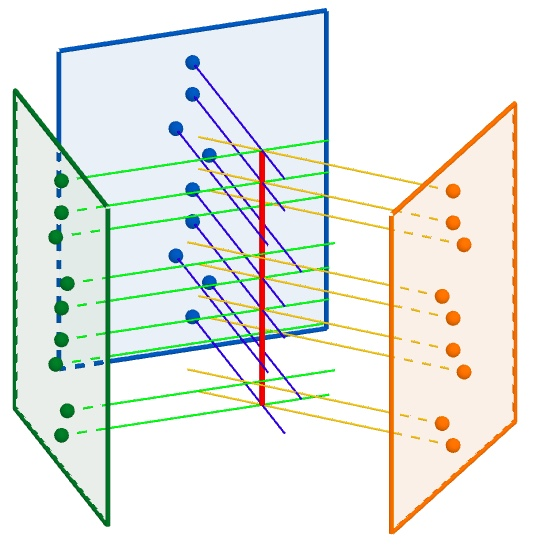
\includegraphics[scale=0.7]{131}

	Рис. 2.7: Построение скрещивающихся прямых через точки множеств.
\end{center}

\newpage
\subsection{Решение}\label{math4:solution}

Алгоритм аналогичен методу 3 \ref{math3:solution}, т.е. имеем задачу по нахождению минимального значения выражения
$$\underset{j=1}{\overset{3}{\sum}} \underset{i=1}{\overset{n_1, n_2, n_3}{\sum}}
\frac{\left(\triangle_{ij}^x (n r_3^j - p r_2^j) - \triangle_{ij}^y (m r_3^j - p r_1^j) + \triangle_{ij}^z (m r_2^j - n r_1^j)\right)^2}{(n r_3^j - p r_2^j)^2 + (p r_1^j - m r_3^j)^2 + (m r_2^j - n r_1^j)^2}$$
по шести параметрам: $m,n,p$ (компоненты вектора искомой прямой) и $x_0, y_0, z_0$ (координаты точки, лежащей на искомой прямой).

\subsection{Погрешность и примеры работы программ}\label{math4:error}

ждет заполнения



\section{Алгоритм сравнения методов и проверки результатов}\label{cha:comparison/sec:alg}

Пусть мы нашли исходный отрезок (прямую). Идея состоит в том, чтобы спроецировать эту прямую на плоскости точек и найти сумму квадратов расстояний от точек до проекций. Сравнение значений данного функционала будет показывать степень отклонения полученной прямой от исходной или степень погрешности метода.\\

Имеем полученную прямую:

\begin{center}
	$\mathit{l}: \; \begin{cases}
		x = x_0 + m \cdot t \\
		y = y_0 + n \cdot t \\
		z = z_0 + p \cdot t
	\end{cases}$, где $t \in \mathbb{R}$ - параметр. 
\end{center}

Проведем через нашу прямую и направления проектирования плоскости:

\begin{center}
	$\pi_1: \; \begin{cases}
		x = x_0 + m \cdot t_1 + r_1^1 \cdot t_2 \\
		y = y_0 + n \cdot t_1 + r_2^1 \cdot t_2 \\
		z = z_0 + p \cdot t_1 + r_3^1 \cdot t_2
	\end{cases}$, где $t_1, t_2 \in \mathbb{R}$ - параметры. 

	\vspace{0.2cm}
	$\pi_2: \; \begin{cases}
		x = x_0 + m \cdot t_1 + r_1^2 \cdot t_2 \\
		y = y_0 + n \cdot t_1 + r_2^2 \cdot t_2 \\
		z = z_0 + p \cdot t_1 + r_3^2 \cdot t_2
	\end{cases}$, где $t_1, t_2 \in \mathbb{R}$ - параметры. 

	\vspace{0.2cm}
	$\pi_3: \; \begin{cases}
		x = x_0 + m \cdot t_1 + r_1^3 \cdot t_2 \\
		y = y_0 + n \cdot t_1 + r_2^3 \cdot t_2 \\
		z = z_0 + p \cdot t_1 + r_3^3 \cdot t_2
	\end{cases}$, где $t_1, t_2 \in \mathbb{R}$ - параметры. 
\end{center}

Аналогично методу 3 \ref{math3:solution}, найдем нормальные уравнения этих плоскостей:

$$\begin{gathered}
	\pi_1: \; A_1 x + B_1 y + C_1 z + D_1 = 0 \\
	\pi_2: \; A_2 x + B_2 y + C_2 z + D_2 = 0 \\
	\pi_3: \; A_3 x + B_3 y + C_3 z + D_3 = 0
\end{gathered}$$
$$\begin{gathered}
	\begin{cases}
		A_1 = \frac{n r_3^1 - p r_2^1}{\sqrt{(n r_3^1 - p r_2^1)^2 + (p r_1^1 - m r_3^1)^2 + (m r_2^1 - n r_1^1)^2}} \\
		B_1 = \frac{p r_1^1 - m r_3^1}{\sqrt{(n r_3^1 - p r_2^1)^2 + (p r_1^1 - m r_3^1)^2 + (m r_2^1 - n r_1^1)^2}} \\
		C_1 = \frac{m r_2^1 - n r_1^1}{\sqrt{(n r_3^1 - p r_2^1)^2 + (p r_1^1 - m r_3^1)^2 + (m r_2^1 - n r_1^1)^2}} \\
		D_1 = \frac{- (n r_3^1 - p r_2^1) x_0 - (p r_1^1 - m r_3^1) y_0 - (m r_2^1 - n r_1^1) z_0}{\sqrt{(n r_3^1 - p r_2^1)^2 + (p r_1^1 - m r_3^1)^2 + (m r_2^1 - n r_1^1)^2}}
	\end{cases} \\
	\begin{cases}
		A_2 = \frac{n r_3^2 - p r_2^2}{\sqrt{(n r_3^2 - p r_2^2)^2 + (p r_1^2 - m r_3^2)^2 + (m r_2^2 - n r_1^2)^2}} \\
		B_2 = \frac{p r_1^2 - m r_3^2}{\sqrt{(n r_3^2 - p r_2^2)^2 + (p r_1^2 - m r_3^2)^2 + (m r_2^2 - n r_1^2)^2}} \\
		C_2 = \frac{m r_2^2 - n r_1^2}{\sqrt{(n r_3^2 - p r_2^2)^2 + (p r_1^2 - m r_3^2)^2 + (m r_2^2 - n r_1^2)^2}} \\
		D_2 = \frac{- (n r_3^2 - p r_2^2) x_0 - (p r_1^2 - m r_3^2) y_0 - (m r_2^2 - n r_1^2) z_0}{\sqrt{(n r_3^2 - p r_2^2)^2 + (p r_1^2 - m r_3^2)^2 + (m r_2^2 - n r_1^2)^2}}
	\end{cases} \\
	\begin{cases}
		A_3 = \frac{n r_3^3 - p r_2^3}{\sqrt{(n r_3^3 - p r_2^3)^2 + (p r_1^3 - m r_3^3)^2 + (m r_2^3 - n r_1^3)^2}} \\
		B_3 = \frac{p r_1^3 - m r_3^3}{\sqrt{(n r_3^3 - p r_2^3)^2 + (p r_1^3 - m r_3^3)^2 + (m r_2^3 - n r_1^3)^2}} \\
		C_3 = \frac{m r_2^3 - n r_1^3}{\sqrt{(n r_3^3 - p r_2^3)^2 + (p r_1^3 - m r_3^3)^2 + (m r_2^3 - n r_1^3)^2}} \\
		D_3 = \frac{- (n r_3^3 - p r_2^3) x_0 - (p r_1^3 - m r_3^3) y_0 - (m r_2^3 - n r_1^3) z_0}{\sqrt{(n r_3^3 - p r_2^3)^2 + (p r_1^3 - m r_3^3)^2 + (m r_2^3 - n r_1^3)^2}}
	\end{cases}
\end{gathered}$$

Найдем плоскости, которым принадлежат множества точек:
$$\begin{gathered}
	w_1: \; r_1^1 x + r_2^1 y + r_3^1 z - (r_1^1 x_1^1 + r_2^1 y_1^1 + r_3^1 z_1^1) = 0 \\
	w_2: \; r_1^2 x + r_2^2 y + r_3^2 z - (r_1^2 x_1^2 + r_2^2 y_1^2 + r_3^2 z_1^2) = 0 \\
	w_3: \; r_1^3 x + r_2^3 y + r_3^3 z - (r_1^3 x_1^3 + r_2^3 y_1^3 + r_3^3 z_1^3) = 0
\end{gathered}$$

В пересечении плоскостей $\pi_1$ и $w_1$, $\pi_2$ и $w_2$, $\pi_3$ и $w_3$ получаем проекции исходного отрезка $l_1, l_2, l_3$ на плоскости множеств $w_1, w_2, w_3$. Тогда расстояния от точек множества $P_i$ до проекции $l_i$ на соответствующую плоскость $w_i$ равно расстоянию от этих точек до плоскости $\pi_i$, проходящую через искомый отрезок $l$.

$$\rho (p_i^j, l_j) = |A_j x_i^j + B_j y_i^j + C_j z_i^j + D_j|$$
где $i$ - номер соответствующей точки множества,

$j$ - номер соответствующей плоскости $\pi_j$.\\
Тогда функционал суммы квадратов расстояний от точек множеств до проекций исходного отрезка равен:
$$\Lambda = \underset{j=1}{\overset{3}{\sum}}\underset{i=1}{\overset{n_1, n_2, n_3}{\sum}}(A_j x_i^j + B_j y_i^j + C_j z_i^j + D_j)^2$$

Итоговый фунционал получается из полученного выше делением на количество исходных множеств точек и на среднее число точек в каждом множетсве.








































\chapter{Вспомогательные алгоритмы}\label{algs}

\section{Построение прямой, аппроксимирующей множество точек}\label{line}

\subsection{Постановка задачи}\label{line:task}

Дано множество из $n$ точек в плоскости или пространстве. Необходимо построить прямую, максимально близкую к заданному множетсву. Меру близости выберем равной корню из суммы квадратов расстояний от точек множества до прямой. Соответственно, необходимо подобрать такие коэффициенты прямой, чтобы для данного набора точек мера на данном множестве и прямой с этими коэффициентами была минимальна.

\begin{figure}[h]
	{ \noindent \centering
	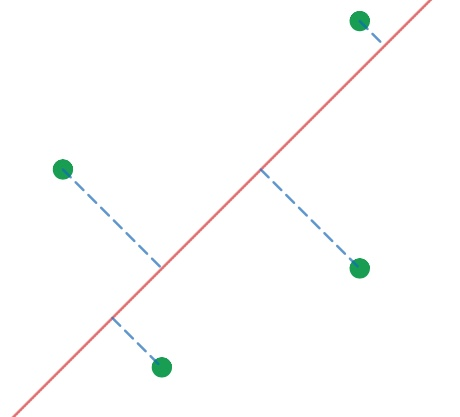
\includegraphics[scale=0.3]{1}
	\caption{Прямая и набор точек в плоскости.}
	}
\end{figure}

\begin{figure}[h]
	{ \noindent \centering
	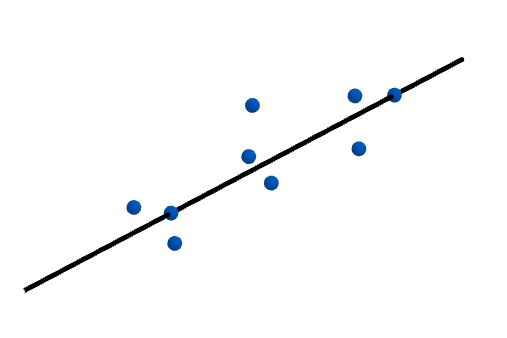
\includegraphics[scale=0.5]{2}
	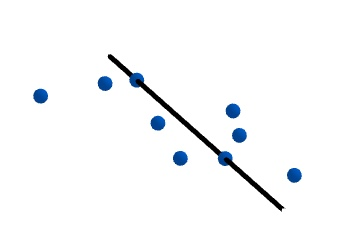
\includegraphics[scale=0.5]{3}
	\caption{Прямая и набор точек в пространстве.}
	}
\end{figure}

\newpage
\subsection{Двумерный случай}\label{line:alg:2dim}

Пусть имеется набор из $n$ точек: $P = \Set{(x_i, y_i)}{i=\ton n}$. 

Будем искать прямую в виде $a \cdot x + b \cdot y + d = 0$, где $a, b, d$ - неизвестные коэффициенты.

По определению расстояние от точки $(x_0, y_0)$ до прямой $ax+by+d=0$ определяется по следующей формуле:

$$\rho (ax+by+d=0, (x_0, y_0)) = \frac{|ax_0+by_0+d|}{\sqrt{a^2+b^2}}$$

Тогда наша мера будет иметь вид:

$$\Lambda (ax+by+d=0,P)=\sqrt{\sum_{i=1}^{n} \frac{(ax_i+by_i+d)^2}{a^2+b^2}}$$

Будем искать нормированное уравнение прямой, которое получается из общего уравнения делением всех членов на $\sqrt{a^2+b^2}$: $a^{'}x+b^{'}y+d^{'}=0$. Тогда расстояние от точки $(x_0,y_0)$ до прямой равно абсолютному значению отклонения и вычисляется по формуле: 

$$\rho (a^{'}x+b^{'}y+d^{'}=0, (x_0, y_0)) = |a^{'}x_0+b^{'}y_0+d^{'}|$$

Тогда наша мера будет иметь вид:

$$\Lambda (a^{'}x+b^{'}y+d^{'}=0,P)=\sqrt{\sum_{i=1}^{n} (a^{'}x_i+b^{'}y_i+d^{'})^2},\;(a^{'})^2+(b^{'})^2=1$$

Будем исследовать не саму меру, а подкоренное выражение, и для простоты будем рассматривать коэффициенты без индексов.

Таким образом, задача свелась к поиску минимального значения выражения $\underset{i=1}{\overset{n}{\sum}}(ax_i+by_i+d)^2$ с ограничением $a^2+b^2=1$.

Будем искать коэффициенты методом Лагранжа. Составим функцию Лагранжа:

$$L(a, b, d, \lambda) = \underset{i=1}{\overset{n}{\sum}}(ax_i+by_i+d)^2 - \lambda (a^2+b^2-1)$$.

Составим систему из четырех уравнений, приравняв к нулю частные производные функции Лагранжа $L(a, b, d, \lambda)$ по $a, b, d$ и $\lambda$:

\begin{center}
	$\begin{cases}
		\frac{\partial}{\partial a} (\underset{i=1}{\overset{n}{\sum}}(ax_i+by_i+d)^2 - \lambda (a^2+b^2-1)) = 0 \\
		\frac{\partial}{\partial b} (\underset{i=1}{\overset{n}{\sum}}(ax_i+by_i+d)^2 - \lambda (a^2+b^2-1)) = 0 \\
		\frac{\partial}{\partial d} (\underset{i=1}{\overset{n}{\sum}}(ax_i+by_i+d)^2 - \lambda (a^2+b^2-1)) = 0 \\
		\frac{\partial}{\partial \lambda} (\underset{i=1}{\overset{n}{\sum}}(ax_i+by_i+d)^2 - \lambda (a^2+b^2-1)) = 0
	\end{cases} \; \Leftrightarrow \;$
\end{center}

\begin{center}
	$\; \Leftrightarrow \;\begin{cases}
		\underset{i=1}{\overset{n}{\sum}}x_i(ax_i+by_i+d) - \lambda a = 0 \\
		\underset{i=1}{\overset{n}{\sum}}y_i(ax_i+by_i+d) - \lambda b = 0 \\
		\underset{i=1}{\overset{n}{\sum}}(ax_i+by_i+d) = 0 \\
		a^2+b^2 = 1
	\end{cases}$
\end{center}

Выразим из третьего уравнения $d$:

$$d = \left(-\frac{\underset{i=1}{\overset{n}{\sum}} x_i}{n}\right) \cdot a + \left(-\frac{\underset{i=1}{\overset{n}{\sum}} y_i}{n}\right) \cdot b$$

Подставим полученное выражение в первые два уравнения:

\begin{center}
	$\begin{cases}
		\underset{i=1}{\overset{n}{\sum}}\left((x_i^2-x_i \cdot\frac{\underset{i=1}{\overset{n}{\sum}} x_i}{n})\cdot a + (x_i y_i - x_i \cdot\frac{\underset{i=1}{\overset{n}{\sum}} y_i}{n})\cdot b\right) - \lambda a = 0\\
		\underset{i=1}{\overset{n}{\sum}}\left((x_i y_i - y_i \cdot\frac{\underset{i=1}{\overset{n}{\sum}} x_i}{n})\cdot a + (y_i^2 - y_i \cdot\frac{\underset{i=1}{\overset{n}{\sum}} y_i}{n})\cdot b\right) - \lambda b = 0\\
	\end{cases}\; \Leftrightarrow \; $
\end{center}

\begin{center}
	$\; \Leftrightarrow \; \begin{pmatrix}
		\underset{i=1}{\overset{n}{\sum}}\left(x_i^2-x_i \cdot\frac{\underset{i=1}{\overset{n}{\sum}} x_i}{n}\right)
		& 
		\underset{i=1}{\overset{n}{\sum}}\left(x_i y_i - x_i \cdot\frac{\underset{i=1}{\overset{n}{\sum}} y_i}{n}\right)
		\\
		\underset{i=1}{\overset{n}{\sum}}\left(x_i y_i - y_i \cdot\frac{\underset{i=1}{\overset{n}{\sum}} x_i}{n}\right)
		&
		\underset{i=1}{\overset{n}{\sum}}\left(y_i^2 - y_i \cdot\frac{\underset{i=1}{\overset{n}{\sum}} y_i}{n}\right)
	\end{pmatrix}\begin{pmatrix}
		a \\ b
	\end{pmatrix} = \lambda \begin{pmatrix}
		a \\ b
	\end{pmatrix}$
\end{center}

\newpage
Таким образом, задача свелась к поиску собственных значений матрицы $A$:

\begin{center}
	$A = \begin{pmatrix}
		\underset{i=1}{\overset{n}{\sum}}x_i^2-\frac{1}{n}\underset{i=1}{(\overset{n}{\sum}} x_i)^2
		& 
		\underset{i=1}{\overset{n}{\sum}}x_i y_i - \frac{1}{n}\underset{i=1}{\overset{n}{\sum}}x_i \underset{i=1}{\overset{n}{\sum}} y_i
		\\
		\underset{i=1}{\overset{n}{\sum}}x_i y_i - \frac{1}{n}\underset{i=1}{\overset{n}{\sum}}x_i \underset{i=1}{\overset{n}{\sum}} y_i
		&
		\underset{i=1}{\overset{n}{\sum}}y_i^2-\frac{1}{n}\underset{i=1}{(\overset{n}{\sum}} y_i)^2
	\end{pmatrix}$
\end{center}

Тем или иным способом, найдем собственные значения. В программе удобно пользоваться методом Якоби, здесь будет изложен прямой метод нахождения собственных значений через характеристический многочлен.

\vspace{0.5cm}
Введем следующие обозначения:

\begin{center}
	$\begin{cases}
		A_{1,1} = \underset{i=1}{\overset{n}{\sum}}x_i^2-\frac{1}{n}\underset{i=1}{(\overset{n}{\sum}} x_i)^2 
		\\
		A_{1,2} = \underset{i=1}{\overset{n}{\sum}}x_i y_i - \frac{1}{n}\underset{i=1}{\overset{n}{\sum}}x_i \underset{i=1}{\overset{n}{\sum}} y_i
		\\
		A_{2,1} = \underset{i=1}{\overset{n}{\sum}}x_i y_i - \frac{1}{n}\underset{i=1}{\overset{n}{\sum}}x_i \underset{i=1}{\overset{n}{\sum}} y_i
		\\
		A_{2,2} = \underset{i=1}{\overset{n}{\sum}}y_i^2-\frac{1}{n}\underset{i=1}{(\overset{n}{\sum}} y_i)^2
	\end{cases} \; \Rightarrow \; A = \begin{pmatrix}
		A_{1,1} & A_{1,2} \\ A_{2,1} & A_{2,2}
	\end{pmatrix}$
\end{center}

Составим характеристическое уравнение:

\begin{center}
	$\begin{vmatrix}
		A_{1,1}-\lambda & A_{1,2} \\ A_{2,1} & A_{2,2}-\lambda
	\end{vmatrix}=0 \; \Rightarrow \; (A_{1,1}-\lambda)(A_{2,2}-\lambda)-A_{1,2} A_{2,1} = 0 \; \Rightarrow \; $
\end{center}

\begin{center}
	$\; \Rightarrow \; \lambda^2 - (A_{1,1}+A_{2,2})\lambda + (A_{1,1} A_{2,2} - A_{1,2} A_{2,1}) = 0 \; \Rightarrow \;$
\end{center}

\begin{center}
	$\; \Rightarrow \; D = (A_{1,1}+A_{2,2})^2-4 (A_{1,1} A_{2,2} - A_{1,2} A_{2,1})$
\end{center}

Будем считать, что в случае решения задачи имеем дело с невырожденным случаем, то $D>0$, тогда:

$$\lambda_1 = \frac{A_{1,1}+A_{2,2} + \sqrt{(A_{1,1}+A_{2,2})^2-4 (A_{1,1} A_{2,2} - A_{1,2} A_{2,1})}}{2}$$

$$\lambda_2 = \frac{A_{1,1}+A_{2,2} - \sqrt{(A_{1,1}+A_{2,2})^2-4 (A_{1,1} A_{2,2} - A_{1,2} A_{2,1})}}{2}$$

\newpage
Получаем две системы:

\begin{center}
	$\begin{cases}
		(A_{1,1} - \lambda_i) a + A_{1,2} b = 0 \\
		A_{2,1} a + (A_{2,2} - \lambda_i) b = 0
	\end{cases},\;i=1,2.$
\end{center}

Данная система однородная, поэтому имеет бесконечное число решений.

Найдем теперь собтвенные векторы. Выразим $a$ через $b$, например, из первых уравнений последних систем:

\begin{center}
	$a = -\frac{A_{1,2}}{A_{1,1}-\lambda_i}b,\;i=1,2$
\end{center}

Положим $b = 1$, тогда $a_i = -\frac{A_{1,2}}{A_{1,1}-\lambda_i},\;i=1,2$.

Уравнение для $d$ через $a$ и $b$ получаем следующее:

\begin{center}
	$d_i = \frac{1}{n}(a_i * \underset{j=1}{\overset{n}{\sum}}x_j + \underset{j=1}{\overset{n}{\sum}}y_j),\;i=1,2$
\end{center}

Далее узнаем значение нашего функционала при данных значениях $a_i, b_i, d$:

\begin{center}
	$L_i (a_i, b = 1, d_i)= \underset{j=1}{\overset{n}{\sum}}(a_i x_j+ y_j + d_i)^2,\;i=1,2$
\end{center}

Выбираем $L = min \{L_1, L_2\}$. Без ограничения общности пусть $L_1 < L_2 \; \Rightarrow \; a = a_1, b = 1, d = d_1$.

Таким образом, итоговые формулы для коэффициентов прмяой получаются следующие:

\begin{center}
	$a = -\frac{A_{1,2}}{A_{1,1}-\lambda_1}, \; b =1, \; d = -\frac{1}{n}(a * \underset{j=1}{\overset{n}{\sum}}x_j + \underset{j=1}{\overset{n}{\sum}}y_j)$
\end{center}.

\newpage
\subsection{Трехмерный случай}\label{line:alg:3dim}

Пусть имеется набор из $n$ точек: $P = \Set{(x_i, y_i, z_i)}{i=\ton n}$. 

Будем искать прямую в параметрическом виде. Пусть $(m, n, p)$ - напрявляющий вектор прямой, $(x_0, y_0, z_0)$ - некоторая точка прямой. Тогда следующая система задает прямую в $\mathbb{R}^3$: 

\begin{center}
	$\mathit{l}: \; \begin{cases}
		x = x_0 + m \cdot t \\
		y = y_0 + n \cdot t \\
		z = z_0 + p \cdot t
	\end{cases}$, где $t \in \mathbb{R}$ - параметр. 
\end{center}

В качестве точки $(x_0, y_0, z_0)$ выбирем центр масс системы данных точек. Таким образом:
$x_0 = \frac{1}{n}\underset{i=1}{\overset{n}{\sum}} x_i, \; y_0 = \frac{1}{n}\underset{i=1}{\overset{n}{\sum}} y_i, \; z_0 = \frac{1}{n}\underset{i=1}{\overset{n}{\sum}} z_i$.

По определению расстояние от точки $M_1$ до прямой $\mathit{l}$ определяется по следующей формуле:

$M_0 (x_0, y_0, z_0)$ - точка на прямой $\mathit{l}$

$\mathit{l} = (m, n, p)$ - напрявляющий вектор прямой

\begin{center}
	$d (M_1, \mathit{l}) = \frac{|[\overline{\mathit{l}}, \overline{M_0 M_1}]|}{|\overline{\mathit{l}}|}$
\end{center}

\begin{center}
	\begin{figure}[h]
	{ 	
		\noindent 
		\centering
		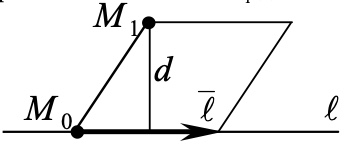
\includegraphics[scale=0.8]{4}
		\caption{Расстояние от точки до прямой.}
	}
\end{figure}
\end{center}

Распишем составляющие элементы формулы для расстояния:

$$|\overline{l}| = \sqrt{m^2 + n^2 + p^2}$$

$$\overline{M_0 M_1} = (x_1 - x_0, y_1 - y_0, z_1 - z_0)$$

$$[\overline{\mathit{l}}, \overline{M_0 M_1}] = \begin{vmatrix}
	\mathbf{i} & \mathbf{j} & \mathbf{k} \\
	m & n & p \\
	x_1 - x_0 & y_1 - y_0 & z_1 - z_0
\end{vmatrix} = $$

$$=\left(\begin{vmatrix}
	n & p \\
	y_1 - y_0 & z_1 - z_0
\end{vmatrix}, -\begin{vmatrix}
	m & p \\
	x_1 - x_0 & z_1 - z_0
\end{vmatrix}, \begin{vmatrix}
	m & n \\
	x_1 - x_0 & y_1 - y_0
\end{vmatrix}\right) = $$

$$= (n (z_1 - z_0) - p (y_1 - y_0), p (x_1 - x_0) - m (z_1 - z_0), m (y_1 - y_0) - n (x_1 - x_0)) = $$

$$ = (n \triangle_{z_1} - p \triangle_{y_1}, p \triangle_{x_1} - m \triangle_{z_1}, m \triangle_{y_1} - n \triangle_{x_1})\text{, где }\begin{cases}
	\triangle_{x_1} = x_1 - x_0 \\
	\triangle_{y_1} = y_1 - y_0 \\
	\triangle_{z_1} = z_1 - z_0
\end{cases}$$

$$|[\overline{\mathit{l}}, \overline{M_0 M_1}]| = \sqrt{(n \triangle_{z_1} - p \triangle_{y_1})^2 + (p \triangle_{x_1} - m \triangle_{z_1})^2 + (m \triangle_{y_1} - n \triangle_{x_1})^2}$$

Тогда формула расстояния принимает вид:

$$d (M_1, \mathit{l}) = \sqrt{\frac{(n \triangle_{z_1} - p \triangle_{y_1})^2 + (p \triangle_{x_1} - m \triangle_{z_1})^2 + (m \triangle_{y_1} - n \triangle_{x_1})^2}{m^2 + n^2 + p^2}}$$

Тогда наша мера примет вид:

$$\Lambda (\mathit{l}, P) = \sqrt{\underset{i=1}{\overset{n}{\sum}} \frac{(n \triangle_{z_i} - p \triangle_{y_i})^2 + (p \triangle_{x_i} - m \triangle_{z_i})^2 + (m \triangle_{y_i} - n \triangle_{x_i})^2}{m^2 + n^2 + p^2} } = $$

$$ = \frac{1}{\sqrt{m^2 + n^2 + p^2}} \sqrt{\underset{i=1}{\overset{n}{\sum}} \left( (n \triangle_{z_i} - p \triangle_{y_i})^2 + (p \triangle_{x_i} - m \triangle_{z_i})^2 + (m \triangle_{y_i} - n \triangle_{x_i})^2 \right)}$$

Будем искать нормированное уравнение прямой, которое получается из общего уравнения делением всех членов на $\sqrt{m^2 + n^2 + p^2}$. Тогда расстояние от точки $(x_0,y_0,z_0)$ до прямой равно абсолютному значению векторного произведения и вычисляется по формуле: 

$$d (M_1, \mathit{l}) = \sqrt{(n \triangle_{z_1} - p \triangle_{y_1})^2 + (p \triangle_{x_1} - m \triangle_{z_1})^2 + (m \triangle_{y_1} - n \triangle_{x_1})^2}$$

Тогда наша мера будет иметь вид:

$$\Lambda (\mathit{l}, P) = \sqrt{\underset{i=1}{\overset{n}{\sum}} \left((n \triangle_{z_i} - p \triangle_{y_i})^2 + (p \triangle_{x_i} - m \triangle_{z_i})^2 + (m \triangle_{y_i} - n \triangle_{x_i})^2 \right)}$$

Будем исследовать не саму меру, а подкоренное выражение.

Таким образом, задача свелась к поиску минимального значения выражения $\underset{i=1}{\overset{n}{\sum}} \left((n \triangle_{z_i} - p \triangle_{y_i})^2 + (p \triangle_{x_i} - m \triangle_{z_i})^2 + (m \triangle_{y_i} - n \triangle_{x_i})^2 \right)$ с ограничением $m^2 + n^2 + p^2=1$.

Будем искать коэффициенты методом Лагранжа. Составим функцию Лагранжа:

$$L(m, n, p, \lambda) = \underset{i=1}{\overset{n}{\sum}} \left((n \triangle_{z_i} - p \triangle_{y_i})^2 + (p \triangle_{x_i} - m \triangle_{z_i})^2 + (m \triangle_{y_i} - n \triangle_{x_i})^2 \right) -$$

$$- \lambda (m^2 + n^2 + p^2-1)$$

Преобразуем выражение под знаком суммы:

$$(n \triangle_{z_i} - p \triangle_{y_i})^2 + (p \triangle_{x_i} - m \triangle_{z_i})^2 + (m \triangle_{y_i} - n \triangle_{x_i})^2 = $$

$$ = n^2 ((\triangle_{x_i})^2 + (\triangle_{z_i})^2) + m^2 ((\triangle_{y_i})^2 + (\triangle_{z_i})^2) + p^2 ((\triangle_{x_i})^2 + (\triangle_{y_i})^2) - $$

$$ - 2 n p \triangle_{y_i} \triangle_{z_i} - 2 m p \triangle_{x_i} \triangle_{z_i} - 2 m n \triangle_{x_i} \triangle_{y_i}$$

Тогда получаем:

$$\underset{i=1}{\overset{n}{\sum}} \left((n \triangle_{z_i} - p \triangle_{y_i})^2 + (p \triangle_{x_i} - m \triangle_{z_i})^2 + (m \triangle_{y_i} - n \triangle_{x_i})^2 \right) = $$

$$ = \underset{i=1}{\overset{n}{\sum}} \Bigl( n^2 ((\triangle_{x_i})^2 + (\triangle_{z_i})^2) + m^2 ((\triangle_{y_i})^2 + (\triangle_{z_i})^2) + p^2 ((\triangle_{x_i})^2 + (\triangle_{y_i})^2) - $$

$$ - 2 n p \triangle_{y_i} \triangle_{z_i} - 2 m p \triangle_{x_i} \triangle_{z_i} - 2 m n \triangle_{x_i} \triangle_{y_i} \Bigl) = $$

$$ = n^2 \underset{i=1}{\overset{n}{\sum}} \left((\triangle_{x_i})^2 + (\triangle_{z_i})^2\right) + m^2 \underset{i=1}{\overset{n}{\sum}} \left((\triangle_{y_i})^2 + (\triangle_{z_i})^2\right) + p^2 \underset{i=1}{\overset{n}{\sum}} \left((\triangle_{x_i})^2 + (\triangle_{y_i})^2\right) - $$

$$ - 2 n p \underset{i=1}{\overset{n}{\sum}} \triangle_{y_i} \triangle_{z_i} - 2 m p \underset{i=1}{\overset{n}{\sum}} \triangle_{x_i} \triangle_{z_i} - 2 m n \underset{i=1}{\overset{n}{\sum}} \triangle_{x_i} \triangle_{y_i}$$

\newpage
Для простоты чтения обозначим коэффициенты в данной формуле следующим образом:

\begin{center}
	$\begin{cases}
		\underset{i=1}{\overset{n}{\sum}} \left((\triangle_{x_i})^2 + (\triangle_{z_i})^2\right) = a_{xz} \\
		\underset{i=1}{\overset{n}{\sum}} \left((\triangle_{y_i})^2 + (\triangle_{z_i})^2\right) = a_{yz} \\
		\underset{i=1}{\overset{n}{\sum}}\left((\triangle_{x_i})^2 + (\triangle_{y_i})^2\right) = a_{xy} \\
		\underset{i=1}{\overset{n}{\sum}} \triangle_{y_i} \triangle_{z_i} = b_{yz} \\
		\underset{i=1}{\overset{n}{\sum}} \triangle_{x_i} \triangle_{z_i} = b_{xz} \\
		\underset{i=1}{\overset{n}{\sum}} \triangle_{x_i} \triangle_{y_i} = b_{xy}
	\end{cases}$
\end{center}

Таким образом, получаем следующую функцию Лагранжа:

$$L(m, n, p, \lambda) = a_{xz} n^2 + a_{yz} m^2 + a_{xy} p^2 - 2 b_{yz} n p - 2 b_{xz} m p  - 2 b_{xy} m n - $$

$$ - \lambda (m^2 + n^2 + p^2-1)$$

Составим систему из четырех уравнений, приравняв к нулю частные производные функции Лагранжа $L(m, n, p, \lambda)$ по $m, n, p$ и $\lambda$:

\begin{center}
	$\begin{cases}
		\frac{\partial}{\partial m} \left(a_{xz} n^2 + a_{yz} m^2 + a_{xy} p^2 - 2 b_{yz} n p - 2 b_{xz} m p  - 2 b_{xy} m n - \lambda (m^2 + n^2 + p^2-1)\right) = 0 \\
		\frac{\partial}{\partial n} \left(a_{xz} n^2 + a_{yz} m^2 + a_{xy} p^2 - 2 b_{yz} n p - 2 b_{xz} m p  - 2 b_{xy} m n - \lambda (m^2 + n^2 + p^2-1)\right) = 0 \\
		\frac{\partial}{\partial p} \left(a_{xz} n^2 + a_{yz} m^2 + a_{xy} p^2 - 2 b_{yz} n p - 2 b_{xz} m p  - 2 b_{xy} m n - \lambda (m^2 + n^2 + p^2-1)\right) = 0 \\
		\frac{\partial}{\partial \lambda} \left(a_{xz} n^2 + a_{yz} m^2 + a_{xy} p^2 - 2 b_{yz} n p - 2 b_{xz} m p  - 2 b_{xy} m n - \lambda (m^2 + n^2 + p^2-1)\right) = 0
	\end{cases} \; \Leftrightarrow \;$
\end{center}

\begin{center}
	$\begin{cases}
		2 a_{yz} m - 2 b_{xz} p - 2 b_{xy} n - 2 \lambda m = 0 \\
		2 a_{xz} n - 2 b_{yz} p - 2 b_{xy} m - 2 \lambda n = 0 \\
		2 a_{xy} p - 2 b_{yz} n - 2 b_{xz} m - 2 \lambda p = 0 \\
		m^2 + n^2 + p^2 = 1
	\end{cases}$
\end{center}

\begin{center}
	$\begin{cases}
		(a_{yz} - \lambda ) m + (-b_{xy}) n + (-b_{xz}) p = 0 \\
		(-b_{xy})m + (a_{xz} - \lambda)n + (-b_{yz})p = 0 \\
		(-b_{xz})m + (-b_{yz})n + (a_{xy} - \lambda)p = 0 \\ 
		m^2 + n^2 + p^2 = 1
	\end{cases}$
\end{center}

Решение первых трех уравнений эквивалентно решению матричного уравнения:

$$\begin{pmatrix}
	a_{yz} - \lambda & -b_{xy} & -b_{xz} \\
	-b_{xy} & a_{xz} - \lambda & -b_{yz} \\
	-b_{xz} & -b_{yz} & a_{xy} - \lambda
\end{pmatrix}\cdot \begin{pmatrix}
	m \\ n \\ p
\end{pmatrix} = 0 \; \Leftrightarrow \; $$

$$\; \Leftrightarrow \; (A - \lambda E)\cdot \begin{pmatrix}
	m \\ n \\ p
\end{pmatrix} = 0,\text{ где } A = \begin{pmatrix}
	a_{yz}  & -b_{xy} & -b_{xz} \\
	-b_{xy} & a_{xz} & -b_{yz} \\
	-b_{xz} & -b_{yz} & a_{xy}
\end{pmatrix}, \; E = \begin{pmatrix}
	1 & 0 & 0 \\
	0 & 1 & 0 \\
	0 & 0 & 1
\end{pmatrix}$$

Тогда задача свелась к поиску собственных значений для матрицы $A$. Тем или иным способом (например, методом Якоби) находим три собственных значения: $\lambda_i,\;i=1,2,3$.

Получаем три системы:

\begin{center}
	$\begin{cases}
		(a_{yz} - \lambda_i ) m + (-b_{xy}) n + (-b_{xz}) p = 0 \\
		(-b_{xy})m + (a_{xz} - \lambda_i)n + (-b_{yz})p = 0 \\
		(-b_{xz})m + (-b_{yz})n + (a_{xy} - \lambda_i)p = 0
	\end{cases}, \; i = 1,2,3$.
\end{center}

Данная система однородная, поэтому имеет бесконечное число решений.

Найдем теперь собтвенные векторы. Выразим $m$ через $n$ и $p$, например, из первых уравнений систем:

$$m = \frac{b_{xy} n + b_{xz} p }{a_{yz} - \lambda_i}, \; i = 1,2,3.$$

Подставим данное выражение во второе и третье уравнения систем:

$$\begin{cases}
	(- \frac{b_{xy}^2}{a_{yz} - \lambda_i} + a_{xz} - \lambda_i) n + (-\frac{b_{xy} b_{xz}}{a_{yz} - \lambda_i} - b_{yz})p = 0 \\
	(-\frac{b_{xz} b_{xy}}{a_{yz} - \lambda_i} - b_{yz}) n + (- \frac{b_{xz}^2}{a_{yz} - \lambda_i} + a_{xy} - \lambda_i) p = 0
\end{cases}, \; i = 1,2,3.$$

Выразим $n$ через $p$ из первого уравнения текущей системы:

$$n = \frac{\frac{b_{xy} b_{xz}}{a_{yz} - \lambda_i} + b_{yz}}{- \frac{b_{xy}^2}{a_{yz} - \lambda_i} + a_{xz} - \lambda_i} p, \; i=1,2,3.$$

Положим $p = 1$. Тогда получаем следующие выражения:

$$n = \frac{\frac{b_{xy} b_{xz}}{a_{yz} - \lambda_i} + b_{yz}}{- \frac{b_{xy}^2}{a_{yz} - \lambda_i} + a_{xz} - \lambda_i}, \; i =1,2,3.$$

$$m = \frac{b_{xy} \left(\frac{\frac{b_{xy} b_{xz}}{a_{yz} - \lambda_i} + b_{yz}}{- \frac{b_{xy}^2}{a_{yz} - \lambda_i} + a_{xz} - \lambda_i}\right) + b_{xz}}{a_{yz} - \lambda_i}, \; i = 1,2,3.$$

Далее узнаем значение нашего функционала при данных значениях $m_i, n_i, p$:

\begin{center}
	$L_i (m_i, n_i, p = 1)= a_{xz} n_i^2 + a_{yz} m_i^2 + a_{xy} - 2 b_{yz} n_i - 2 b_{xz} m_i  - 2 b_{xy} m_i n_i, \;i=1,2,3.$
\end{center}

Выбираем $L = min \{L_1, L_2, L_3\}$. Без ограничения общности пусть $L_1 < L_2 < L_3 \; \Rightarrow \; m = m_1, n = n_1, p = 1$.

Таким образом, итоговые формулы для коэффициентов прмяой получаются следующие:

$$\begin{cases}
	m = \frac{b_{xy} \left(\frac{\frac{b_{xy} b_{xz}}{a_{yz} - \lambda_1} + b_{yz}}{- \frac{b_{xy}^2}{a_{yz} - \lambda_1} + a_{xz} - \lambda_1}\right) + b_{xz}}{a_{yz} - \lambda_1} \\
	n = \frac{\frac{b_{xy} b_{xz}}{a_{yz} - \lambda_1} + b_{yz}}{- \frac{b_{xy}^2}{a_{yz} - \lambda_1} + a_{xz} - \lambda_1} \\
	p = 1 \\
	(x_0, y_0, z_0)\text{ - центр масс системы:} \\
	x_0 = \frac{1}{n}\underset{i=1}{\overset{n}{\sum}} x_i, \; y_0 = \frac{1}{n}\underset{i=1}{\overset{n}{\sum}} y_i, \; z_0 = \frac{1}{n}\underset{i=1}{\overset{n}{\sum}} z_i
\end{cases}$$

\newpage
\subsection{Примеры работы программ}\label{line:application}

\subsubsection{Двумерный случай}\label{line:application:2dim}

\begin{figure}[h]
	{ \noindent \centering
	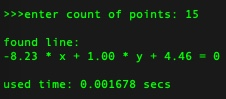
\includegraphics[scale=1]{5}
	\caption{Пример ввода данных и выдачи результата.}
	}
\end{figure}

\begin{figure}[h]
	{ \noindent \centering
	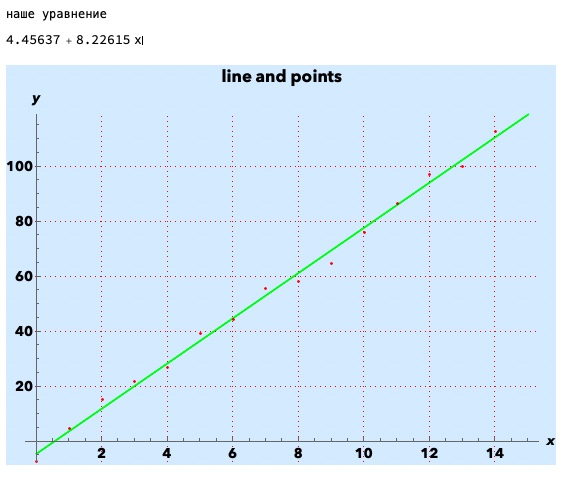
\includegraphics[scale=0.7]{6}
	\caption{Визуализация результата в Wolfram Mathematica.}
	}
\end{figure}

\newpage
\subsubsection{Трехмерный случай}\label{line:application:3dim}

\begin{figure}[h]
	{ \noindent \centering
	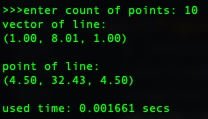
\includegraphics[scale=1]{7}
	\caption{Пример ввода данных и выдачи результата.}
	}
\end{figure}

\begin{figure}[h]
	{ \noindent \centering
	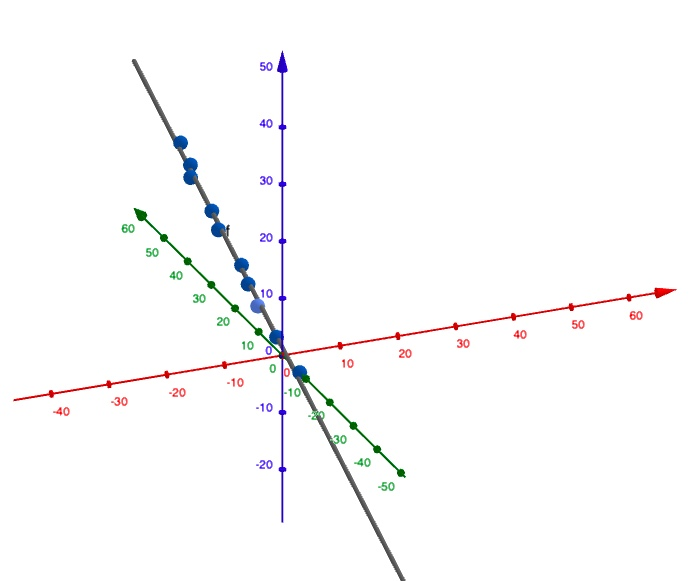
\includegraphics[scale=0.6]{8}
	\caption{Визуализация результата в GeoGebra3D.}
	}
\end{figure}
\section{Построение прямой (точки), минимально удаленной от множества плоскостей (отрезков)}\label{plane}

\subsection{Постановка задачи}\label{plane:task}

Дано множество из $n$ отрезков на плоскости или $n$ плоскостей в пространстве. Необходимо найти точку на плоскоти, минимально удаленную от заданных отрезков, или прямую в пространстве, минимально удаленную от заданных плоскостей. Меру близости на плоскости выберем равной корню из суммы квадратов расстояний от точки до прямых, содержащих отрезки. Меру близости в пространстве выберем равной корню из суммы квадратов расстояний от прямой до плоскостей: в случае параллельности или совпадения прямой и плоскости берется расстояние от любой точки прямой до плоскости, а в случае пересечения берется расстояние от плоскости до точки прямой, ближайщей к этой плоскости внутри призмы, объемлющей рассматриваемый компакт пространства. 

\begin{figure}[h]
	{ \noindent \centering
	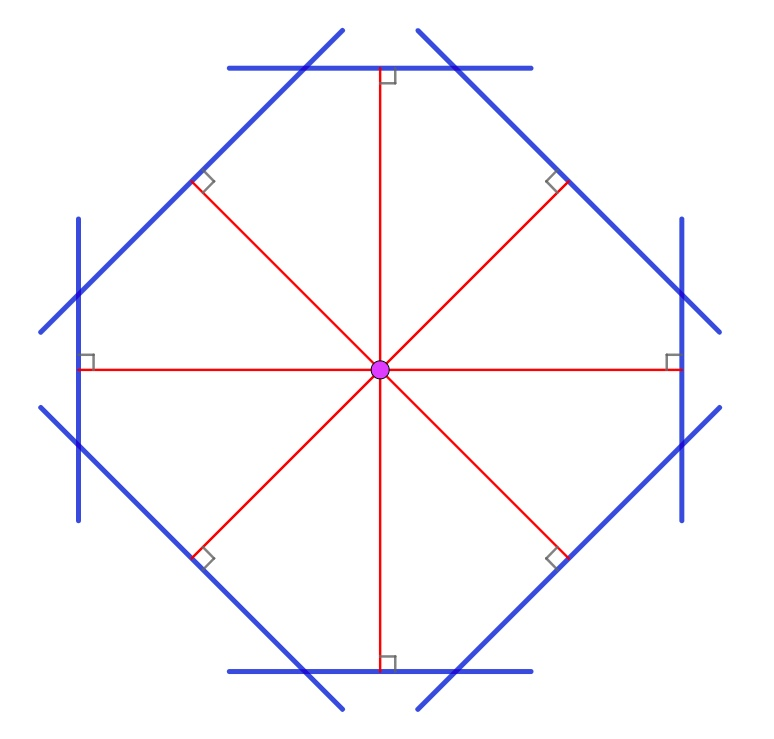
\includegraphics[scale=0.5]{plane01}
	\caption{Точка и множество отрезков на плоскости.}
	}
\end{figure}

\begin{figure}[h]
	{ \noindent \centering
	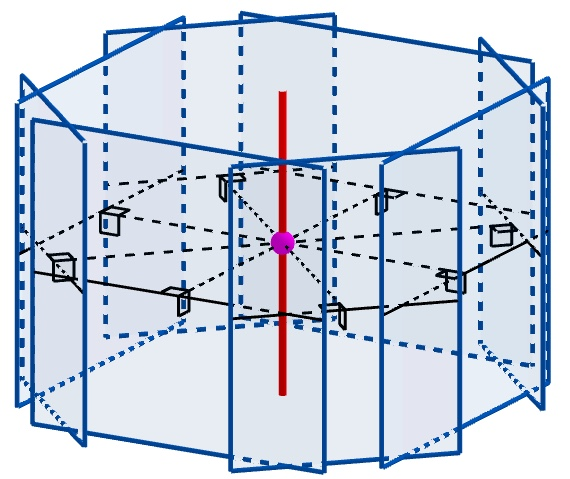
\includegraphics[scale=0.7]{plane02}
	\caption{Отрезок и множество плоскостей в пространстве.}
	}
\end{figure}

\newpage
\subsection{Двумерный случай}\label{plane:alg:2dim}

Пусть дан набор из $n-1$ отрезков в виде набора пар их вершин: 
$$S = \Set{\;((x_i, y_i), (x_{i+1}, y_{i+1}))\;}{i = \ton n-1}$$

Таким образом, у нас имеется точка, через которую проходит каждый отрезок, и направление прямой, на которой лежит каждый отрезок, и можно переписать множетсво отрезков следующим образом:
$$\begin{gathered}
	S^* =\Set{\; \left( (x_i^{(c)}, y_i^{(c)}), (l_i^x, l_i^y) \right) \;}{i= \ton n-1} \\
	x_i^{(c)} = \frac{x_i + x_{i+1}}{2}, \; y_i^{(c)} = \frac{y_i + y_{i+1}}{2} \\
	l_i^x = x_{i+1} - x_i, \; l_i^y = y_{i+1} - y_i
\end{gathered}$$

Отнормируем напрявляющие векторы прямых, содержащих отрезки:
$$\tilde{l}_i^x = \frac{x_{i+1} - x_i}{\sqrt{(x_{i+1} - x_i)^2+(y_{i+1} - y_i)^2}}, \; \tilde{l}_i^y = \frac{y_{i+1} - y_i}{\sqrt{(x_{i+1} - x_i)^2+(y_{i+1} - y_i)^2}}$$

\newpage
Тогда нормальные уравнения этих прямых будут иметь вид:

$$\begin{gathered}
	a_i x + b_i y + c_i = 0, \; i = \ton n-1 \\
	 a_i = \tilde{l}_i^y, \; b_i = -\tilde{l}_i^x, \; c_i = - (a_i x_i^{(c)} + b_i y_i^{(c)})
\end{gathered}$$

\vspace{0.5cm}
Будем искать точку $O = (x_0, y_0)$, наименее удаленную от данного множества отрезков.

Формула расстояния от точки прямой, содержащей каждый отрезок:
$$\rho (O, l_i) = \frac{|a_i x_0 + b_i y_0 + c_i|}{\sqrt{a_i^2+b_i^2}} = |a_i x_0 + b_i y_0 + c_i|, \; i = \ton n-1$$

Наша мера будет иметь вид:
$$L_0(x_0, y_0) = \sqrt{\underset{i=1}{\overset{n-1}{\sum}}(a_i x_0 + b_i y_0 + c_i)^2}$$

Будем работать не с этой меру, а с выражением под корнем (в силу монотонности функции корня это эквивалентная задача), т.е. имеем функционал:
$$L (x_0, y_0) = \underset{i=1}{\overset{n-1}{\sum}}(a_i x_0 + b_i y_0 + c_i)^2$$

Таким образом, задача свелась к поиску минимального значения выражения $L(x_0, y_0)$.

Составим систему из двух уравнений, приравняв к нулю частные производные функционала $L(x_0, y_0)$ по $x_0$ и $y_0$:
$$\begin{cases}
	\frac{\partial}{\partial x_0} \underset{i=1}{\overset{n-1}{\sum}}(a_i x_0 + b_i y_0 + c_i)^2 = \underset{i=1}{\overset{n-1}{\sum}} \left( \frac{\partial}{\partial x_0}(a_i x_0 + b_i y_0 + c_i)^2 \right) = 0 \\
	\frac{\partial}{\partial y_0} \underset{i=1}{\overset{n-1}{\sum}}(a_i x_0 + b_i y_0 + c_i)^2 = \underset{i=1}{\overset{n-1}{\sum}} \left( \frac{\partial}{\partial y_0}(a_i x_0 + b_i y_0 + c_i)^2 \right)= 0
\end{cases} \; \Leftrightarrow$$
$$\Leftrightarrow \; \begin{cases}
	\underset{i=1}{\overset{n-1}{\sum}} \left( 2 a_i (a_i x_0 + b_i y_0 + c_i) \right) = 0 \\
	\underset{i=1}{\overset{n-1}{\sum}} \left( 2 b_i (a_i x_0 + b_i y_0 + c_i) \right) = 0
\end{cases} \Leftrightarrow$$
$$ \Leftrightarrow \;  \begin{cases}
	\left( \underset{i=1}{\overset{n-1}{\sum}} a_i^2 \right) x_0 + \left( \underset{i=1}{\overset{n-1}{\sum}} a_i b_i \right) y_0 + \underset{i=1}{\overset{n-1}{\sum}} a_i c_i = 0 \\
	\left( \underset{i=1}{\overset{n-1}{\sum}} a_i b_i \right) x_0 + \left( \underset{i=1}{\overset{n-1}{\sum}} b_i^2 \right) y_0 + \underset{i=1}{\overset{n-1}{\sum}} b_i c_i = 0
\end{cases}\eqno(*)$$

Для выяснения совместности системы воспользуемся теоремой Кронекера-Капелли и следствием из нее:
\begin{theorem}[\red{Кронекера-Капелли}]\label{plane/the:1}
	Система линейных алгебраических уравнений совместна тогда и только тогда, когда ранг матрицы системы равен рангу расширенной матрицы системы, т.е. $rk A = rk \tilde{A}$
\end{theorem}

\begin{conseq}\label{plane/conseq:1}
	Из теоремы Кронекера-Капелли получаем утвреждения:
	\begin{enumerate}
		\item если $rk A \not = rk \tilde{A}$, то СЛАУ несовместна
		\item если $rk A = rk \tilde{A} < n$, то СЛАУ имеет бесконечное число решений
		\item если $rk A = rk \tilde{A} = n$, то СЛАУ имеет ровно одно решение
	\end{enumerate}
\end{conseq}

В нашем случае имеем:
$$n=2, \; A = \begin{pmatrix}
	\underset{i=1}{\overset{n-1}{\sum}} a_i^2 & \underset{i=1}{\overset{n-1}{\sum}} a_i b_i\\
	\underset{i=1}{\overset{n-1}{\sum}} a_i b_i & \underset{i=1}{\overset{n-1}{\sum}} b_i^2
\end{pmatrix}, \; \tilde{A} = \begin{pmatrix}
	\underset{i=1}{\overset{n-1}{\sum}} a_i^2 & \underset{i=1}{\overset{n-1}{\sum}} a_i b_i & -\underset{i=1}{\overset{n-1}{\sum}} a_i c_i\\
	\underset{i=1}{\overset{n-1}{\sum}} a_i b_i & \underset{i=1}{\overset{n-1}{\sum}} b_i^2 & -\underset{i=1}{\overset{n-1}{\sum}} b_i c_i
\end{pmatrix}$$

Таким образом, получаем:
\begin{itemize}
 	\item 
 		если $rk A = rk \tilde{A} = 1 < 2$, т.е. $\frac{\underset{i=1}{\overset{n-1}{\sum}} a_i^2}{\underset{i=1}{\overset{n-1}{\sum}} a_i b_i}=\frac{\underset{i=1}{\overset{n-1}{\sum}} a_i b_i}{\underset{i=1}{\overset{n-1}{\sum}} b_i^2}=\frac{\underset{i=1}{\overset{n-1}{\sum}} a_i c_i}{\underset{i=1}{\overset{n-1}{\sum}} b_i c_i}$, то система имеет бесконечное число решение, т.е. существует прямая, равноудаленная от исходного множества отрезков (прямых) - любое из уравнений системы $(*)$
 	\item 
 		если $rk A \not = rk \tilde{A} \; \Leftrightarrow \; rk A = 1, rk \tilde{A} = 2$, т.е. $\frac{\underset{i=1}{\overset{n-1}{\sum}} a_i^2}{\underset{i=1}{\overset{n-1}{\sum}} a_i b_i}=\frac{\underset{i=1}{\overset{n-1}{\sum}} a_i b_i}{\underset{i=1}{\overset{n-1}{\sum}} b_i^2}\not=\frac{\underset{i=1}{\overset{n-1}{\sum}} a_i c_i}{\underset{i=1}{\overset{n-1}{\sum}} b_i c_i}$, то система несовместна (нет решений), но это невозможно, докажем это.
 		Пусть $a = (a_1, \dots, a_{n-1}), \; b = (b_1, \dots, b_{n-1})$. Тогда матрица $A$ является матрицей скалярных произведений векторов $a$ и $b$:
 		$$A = 
 		\begin{pmatrix}
 			(a,a) & (a,b) \\
 			(a,b) & (b,b)
 		\end{pmatrix}$$
 		Из неравенства Коши-Буняковского знаем, что произведение квадратов норм векторов не меньше, чем произведение скалярных произведений этих векторов, причем равенство достигается, только если векторы пропорциональны. Таким образом, если они не пропорциональны, то $rk A = rk \tilde{A} = 2$, а если пропорциональны, то $rk A = rk \tilde{A} = 1$, т.е. случай $rk A \not = rk \tilde{A}$ невозможен.
 	\item
 		если $rk A = rk \tilde{A} = 2$, т.е. $\begin{vmatrix}
			\underset{i=1}{\overset{n-1}{\sum}} a_i^2 & \underset{i=1}{\overset{n-1}{\sum}} a_i b_i\\
			\underset{i=1}{\overset{n-1}{\sum}} a_i b_i & \underset{i=1}{\overset{n-1}{\sum}} b_i^2
		\end{vmatrix} \not = 0$, то система имеет единственное решение (одну точку):
		$$\begin{cases}
		x_0 = \frac{\left( \underset{i=1}{\overset{n-1}{\sum}} b_i^2 \right) \left( \underset{i=1}{\overset{n-1}{\sum}} a_i c_i \right) - \left( \underset{i=1}{\overset{n-1}{\sum}} a_i b_i \right) \left( \underset{i=1}{\overset{n-1}{\sum}} b_i c_i \right)}{\left( \underset{i=1}{\overset{n-1}{\sum}} a_i b_i \right)^2 - \left( \underset{i=1}{\overset{n-1}{\sum}} a_i^2 \right)\left( \underset{i=1}{\overset{n-1}{\sum}} b_i^2 \right)} \\
		y_0 = \frac{\left( \underset{i=1}{\overset{n-1}{\sum}} a_i^2 \right) \left( \underset{i=1}{\overset{n-1}{\sum}} b_i c_i \right) - \left( \underset{i=1}{\overset{n-1}{\sum}} a_i b_i \right) \left( \underset{i=1}{\overset{n-1}{\sum}} a_i c_i \right)}{\left( \underset{i=1}{\overset{n-1}{\sum}} a_i b_i \right)^2 - \left( \underset{i=1}{\overset{n-1}{\sum}} a_i^2 \right)\left( \underset{i=1}{\overset{n-1}{\sum}} b_i^2 \right)}
	\end{cases}$$
 \end{itemize}

\newpage
\subsection{Трехмерный случай}\label{plane:alg:3dim}

\subsubsection{Случай параллельности плоскостей и прямой}\label{plane:alg:3dim:paral}

Пусть дан набор из $n$ плоскостей в виде набора пар их векторов нормали и точек, принадлежащих им: 
$$S = \Set{\;((x_i, y_i, z_i), (m_i, n_i, p_i))\;}{i = \ton n}$$

По смыслу задачи координата $l_i$ для всех плоскостей равна 0, или существует афинная замена координат, приводящая к такой ситуации, т.е. пользуемся алгоритмом замены координат \ref{coords:alg:3dim}. Таким образом, имеем следующий набор:
$$S = \Set{\;((x_i, y_i, z_i), (m_i, n_i, 0))\;}{i = \ton n}$$

Отнормируем вектора нормали плоскостей:
$$\tilde{m_i} = \frac{m_i}{\sqrt{m_i^2+n_i^2}}, \; \tilde{n_i} = \frac{n_i}{\sqrt{m_i^2+n_i^2}}$$

Тогда уравнения наших плоскостей имеют вид:
$$\tilde{m_i} (x - x_i) + \tilde{n_i} (y - y_i) = 0$$

Если рассматривать обычное уравнение плоскости, то получаем следующие тождества:
$$\begin{gathered}
	A x + B y + C z + D = 0 \\
	A = \tilde{m_i}, \; B = \tilde{n_i}, \; C = 0, \; D = -\tilde{m_i} x_i - \tilde{n_i} y_i
\end{gathered}$$

Будем искать прямую $l$, наименее удаленную от данного множества плоскостей:
\begin{center}
	$\mathit{l}: \; \begin{cases}
		x = x_0 + m \cdot t \\
		y = y_0 + n \cdot t \\
		z = z_0 + p \cdot t
	\end{cases}$, где $t \in \mathbb{R}$ - параметр. 
\end{center}

Т.к. все плоскости параллельны оси OZ, то и искомая прямая будет параллельна ей, т.е. направляющий вектор будет равен $(0,0,1)$. Таким образом, задача свелась к нахождению точки, наименее удаленной от множества данных плоскостей, в любой плоскости, например, $z = 0$. В пересечении плоскости $z=0$ и исходного набора плоскостей получаем набор отрезков (прямых), и задача полностью свелась к двумерному случаю \ref{plane:alg:2dim}.

\subsubsection{Случай непараллельности плоскостей и прямой}\label{plane:alg:3dim:neparal}

Аналогично случаю параллельности \ref{plane:alg:3dim:paral} имеем нормальные уравнения плоскостей:
$$\begin{gathered}
	\pi_i: \; A_i x + B_i y + C_i z + D_i = 0 \\
	A_i = \frac{m_i}{\sqrt{m_i^2 + n_i^2 + p_i^2}}, \;
	B_i = \frac{n_i}{\sqrt{m_i^2 + n_i^2 + p_i^2}} \\
	C_i = \frac{p_i}{\sqrt{m_i^2 + n_i^2 + p_i^2}}, \;
	D_i = -\frac{m_i x_i + n_i y_i + p_i z_i}{\sqrt{m_i^2 + n_i^2 + p_i^2}}
\end{gathered}$$

Будем рассматривать задачу внутри объемлющей призмы, ограниченной $z_{min}$ и $z_{max}$, т.е. концы искомого отрезка будем искать на этих плоскостях, ограничивающий призму <<сверху>> и <<снизу>>. Наша прямая будет определяться точками $P_1 = (x_1, y_1, z_{min})$ и $P_2 = (x_2, y_2, z_{max})$.\\

% Одну из точек прямой можно зафиксировать. Найдем среднее значение $z_{mid}$ среди всех диапазона значений $z$. Проведем плоскость, параллельную плоскости OXY: $z = z_{mid}$. В пересечении этой плоскости с исходными имеем прямые, решаем двумерную задачу нахожения точки, наименее удаленной от прямых \ref{plane:alg:2dim}.

Будем искать расстояние от прямой до каждой их плоскостей следующим образом: пусть $d_1 = \rho \left( P_1, \pi_i \right), \;\; d_2 = \rho \left( P_2, \pi_i \right)$, тогда $\rho (l, \pi_i) = \frac{d_1^2 + d_2^2 + d_1 d_2}{3}$.\\

$$\begin{gathered}
	d_{1i} = \rho \left( P_1, \pi_i \right) = |A_i x_1 + B_i y_1 + C_i z_{min} + D_i| \\
	d_{2i} = \rho \left( P_2, \pi_i \right) = |A_i x_2 + B_i y_2 + C_i z_{max} + D_i|\\
	\rho (l, \pi_i) = \frac{d_1^2 + d_2^2 + d_1 d_2}{3} = \\
	= \frac{\left( A_i x_1 + B_i y_1 + C_i z_{min} + D_i \right)^2 + \left( A_i x_2 + B_i y_2 + C_i z_{max} + D_i \right)^2}{3} + \\
	+ \frac{|A_i x_1 + B_i y_1 + C_i z_{min} + D_i||A_i x_2 + B_i y_2 + C_i z_{max} + D_i|}{3}
\end{gathered}$$

В плоскостях $z = z_{min}$ и $z = z_{max}$ будем искать точки $P_1$ и $P_2$ так, чтобы они были наименее удалены от исходных плоскостей $\pi_i$.

$$d_{ji} = \rho \left( P_1, \pi_i \right) = |A_i x_j + B_i y_j + C_i z_j + D_i|, \;\; j = 1,2, \;\; z_j = \begin{cases}
	z_{min}, \; j = 1 \\
	z_{max}, \; j = 2
\end{cases}$$

Тогда функционал имеет вид:
$$\Lambda = \underset{i=1}{\overset{n}{\sum}}(A_i x_j + B_i y_j + C_i z_{min} + D_i)^2$$

Найдем частные производные функционала по $x_j$ и $y_j$:
$$\begin{cases}
	\frac{\partial}{\partial x_j} \underset{i=1}{\overset{n}{\sum}}(A_i x_j + B_i y_j + C_i z_j + D_i)^2 = 0 \\
	\frac{\partial}{\partial y_j} \underset{i=1}{\overset{n}{\sum}}(A_i x_j + B_i y_j + C_i z_j + D_i)^2 = 0
\end{cases}\; \Rightarrow \; $$
$$\begin{gathered}
	\begin{cases}
		\underset{i=1}{\overset{n}{\sum}}\frac{\partial}{\partial x_j}(A_i x_j + B_i y_j + C_i z_j + D_i)^2 = 0 \\
		\underset{i=1}{\overset{n}{\sum}}\frac{\partial}{\partial y_j}(A_i x_j + B_i y_j + C_i z_j + D_i)^2 = 0
	\end{cases} \Rightarrow \; 
	\begin{cases}
		\underset{i=1}{\overset{n}{\sum}}2A_i (A_i x_j + B_i y_j + C_i z_j + D_i) = 0 \\
		\underset{i=1}{\overset{n}{\sum}}2B_i (A_i x_j + B_i y_j + C_i z_j + D_i) = 0
	\end{cases}\\
	\; \Rightarrow \begin{cases}
		\left( \underset{i=1}{\overset{n}{\sum}} A_i^2 \right) x_j + \left( \underset{i=1}{\overset{n}{\sum}} A_i B_i \right) y_j + \underset{i=1}{\overset{n}{\sum}}A_i (C_i z_j + D_i) = 0 \\
		\left( \underset{i=1}{\overset{n}{\sum}} A_i B_i \right) x_j + \left( \underset{i=1}{\overset{n}{\sum}} B_i^2 \right) y_j + \underset{i=1}{\overset{n}{\sum}}B_i (C_i z_j + D_i) = 0
	\end{cases}
\end{gathered}$$

Введем обозначения:
$$\begin{cases}
	a_{11} = \underset{i=1}{\overset{n}{\sum}} A_i^2 \\
	a_{12} = \underset{i=1}{\overset{n}{\sum}} A_i B_i \\
	a_{22} = \underset{i=1}{\overset{n}{\sum}} B_i^2 \\
	b_1 = \underset{i=1}{\overset{n}{\sum}}A_i (C_i z_j + D_i) \\
	b_2 = \underset{i=1}{\overset{n}{\sum}}B_i (C_i z_j + D_i)
\end{cases}$$

Если система невырождена, то получаем решение:
$$\begin{cases}
	x_j = \frac{a_{22} b_1 - a_{12} b_2}{a_{12}^2 - a_{11}a_{22}} \\
	y_j = \frac{a_{11} b_2 - a_{12} b_1}{a_{12}^2 - a_{11}a_{22}}
\end{cases}$$

Таким образом, имеем две точки, по которым однозначно определяется искомая прямая.

% \newpage
% \subsection{Примеры работы программ}\label{plane:application}

% \subsubsection{Двумерный случай}\label{plane:application:2dim}

% ждет заполнения

% \newpage
% \subsubsection{Трехмерный случай}\label{plane:application:3dim}

% ждет заполнения
\newpage
\section{Замена координат}\label{coords}

\subsection{Постановка задачи}\label{coords:task}

На плоскости или в пространстве заданы некоторые геометрические объекты в своем базисе. Необходимо найти координат этих объектов при замене базиса на новый.

\begin{figure}[h]
	{ \noindent \centering
	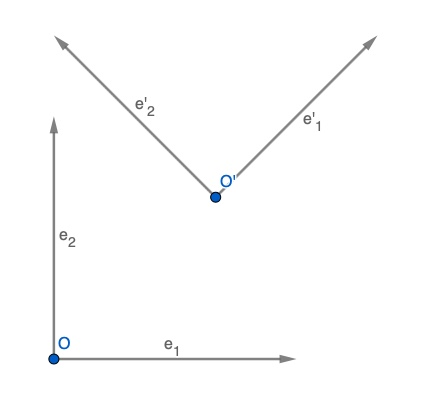
\includegraphics[scale=0.5]{cords2d}
	\caption{Два базиса на плоскости.}
	}
\end{figure}

\begin{figure}[h]
	{ \noindent \centering
	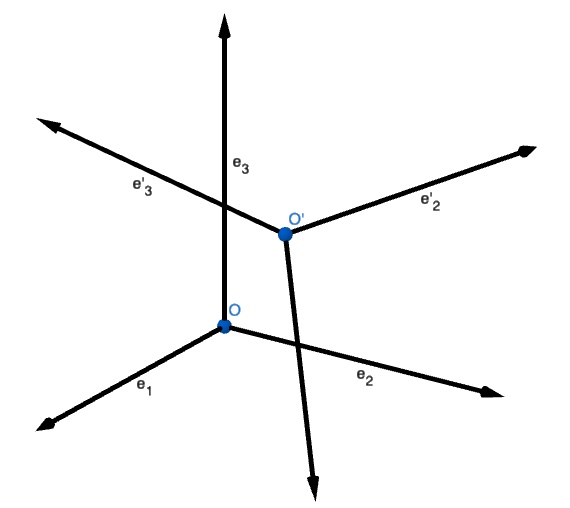
\includegraphics[scale=0.5]{cords3d}
	\caption{Два базиса в пространстве.}
	}
\end{figure}

\newpage
\subsection{Двумерный случай}\label{coords:alg:2dim}

Рассмотрим ортогональную матрицу как матрицу перехода от ортонормированного базиса $e_1, e_2$ к ортонормированному базису $e'_1, e'_2$. Тогда вектор $e'_1$ имеет координаты $(\cos \varphi, \sin \varphi)$ для некоторого $\varphi$. Перпендикулярные ему векторы единичной длины (таких два) равны $(\mp \sin \varphi, \pm \cos \varphi)$.\\

Таким образом, ортогональные матрицы 2x2 имеют один из следующих видов:
$$C = 
\begin{pmatrix}
	\cos \varphi & -\sin \varphi \\
	\sin \varphi & \cos \varphi
\end{pmatrix}, \; C = 
\begin{pmatrix}
	\cos \varphi & \sin \varphi \\
	\sin \varphi & -\cos \varphi
\end{pmatrix}$$

Угол $\varphi$ можно считать принадлежащим $[0, 2\pi)$.\\

Координаты точки в старой и новой с. к. связаны соотношениями:
$$\begin{pmatrix}
	x \\ y
\end{pmatrix} = C \begin{pmatrix}
	x' \\ y'
\end{pmatrix} + \begin{pmatrix}
	x_0 \\ y_0
\end{pmatrix}$$
где $C$ - матрица перехода от старого базиса к новому,

\hspace{0.4cm}$(x,y)$ и $(x', y')$ - координаты точки в старой и новой с.к.

\hspace{0.4cm}$(x_0, y_0)$ - координаты нового начала координат $O'$ в старой с.к.\\

Координаты векторов в старой и новой с. к. связаны соотношениями:
$$\begin{pmatrix}
	\alpha \\ \beta
\end{pmatrix} = C \begin{pmatrix}
	\alpha' \\ \beta'
\end{pmatrix}$$

Чтобы найти обратную замену, необходимо умножить на $C^{-1}$, а для ортогональных матриц $C^{-1} = C^T$. Таким образом:
$$\begin{pmatrix}
	x' \\ y'
\end{pmatrix} = C^T \begin{pmatrix}
	x \\ y
\end{pmatrix} - C^T \begin{pmatrix}
	x_0 \\ y_0
\end{pmatrix}$$

\newpage
\subsection{Трехмерный случай}\label{coords:alg:3dim}

Рассмотрим переход от прямоугольной системы координат $O e_1 e_2 e_3$ к другой прямоугольной системе координат $O e'_1 e'_2 e'_3$.

При коолинеарности одного из базисных векторов, например, $e_3$ первого репера и одного базисного вектора, например, $e'_3$ из второго репера замена сводится к замене координат на плоскости с определителем соответствующего знака в зависимости от направленности коллинерных векторов.

Теперь будем считать, что все векторы неколлинеарны, в частности, $e_3$ и $e'_3$ неколлинеарны:
$$\begin{gathered}
	e_3 \text{ - вектор нормали к плоскости } O e_1 e_2 \\
	e'_3 \text{ - вектор нормали к плоскости } O' e'_1 e'_2
\end{gathered}$$

Определим вектор $f := \frac{[e_3, e'_3]}{||[e_3, e'_3]||}$ - это направляющий вектор прямой пересечения плоскостей $O e_1 e_2$ и $O' e'_1 e'_2$.

Также определим \textit{углы Эйлера}:
\begin{itemize}
	\item[$\bullet$] угол $\varphi$ - это угол от $e_1$ к $f$, $\varphi \in [0, 2\pi)$
	\item[$\bullet$] угол $\theta$ - это угол от $e_3$ к $e'_3$, $\theta \in [0, \pi]$
	\item[$\bullet$] угол $\psi$ - это угол от $f$ к $e'_1$, $\psi \in [0, 2\pi)$
\end{itemize}

Будем последовательно производить замены координат: повороты в соответствующих плоскостях.

\begin{enumerate}
	\item Переход от $O e_1 e_2 e_3$ к $O f g e_3$ с сохранением ориентации - это вращение вокруг $e_3$ на угол $\phi$. Соответствующая матрица перехода имеет вид:
	$$C_1 = \begin{pmatrix}
		\cos \varphi & -\sin \varphi & 0 \\
		\sin \varphi & \cos \varphi & 0 \\
		0 & 0 & 1
	\end{pmatrix}$$
	\item Проведем вращение вокруг $f$ так, чтобы $e_3$ совместился с $e'_3$ - это вращение на угол $\theta$ (в силу определения $f$). Получаем переход к реперу $O f h e'_3$, причем плоскости $O f h$ и $O e'_1 e'_2$ совпадают. Соответствующая матрица перехода имеет вид:
	$$C_2 = \begin{pmatrix}
		1 & 0 & 0 \\
		0 &\cos \theta & -\sin \theta\\
		0 & \sin \theta & \cos \theta
	\end{pmatrix}$$
	\item Проведем вращение вокруг $e'_3$ в плоскости $O e'_1 e'_2$ для совмещения $f$ и $e'_1$. При этом в силу согласованности ориентаций образ $e_2$ перейдет в $e'_2$.
	Соответствующая матрица перехода имеет вид:
	$$C_3 = \begin{pmatrix}
		\cos \psi & -\sin \psi & 0 \\
		\sin \psi & \cos \psi & 0 \\
		0 & 0 & 1
	\end{pmatrix}$$
\end{enumerate}

Тогда результирущая матрица перехода от базиса $e_1 e_2 e_3$ к $e'_1 e'_2 e'_3$ равна:
$$\begin{gathered}
	C = C_1 C_2 C_3 = \begin{pmatrix}
		\cos \varphi & -\sin \varphi & 0 \\
		\sin \varphi & \cos \varphi & 0 \\
		0 & 0 & 1
	\end{pmatrix} 
	\begin{pmatrix}
		1 & 0 & 0 \\
		0 &\cos \theta & -\sin \theta\\
		0 & \sin \theta & \cos \theta
	\end{pmatrix}
	\begin{pmatrix}
		\cos \psi & -\sin \psi & 0 \\
		\sin \psi & \cos \psi & 0 \\
		0 & 0 & 1
	\end{pmatrix} = \\
	= \begin{pmatrix}
		\cos \varphi \cos \psi - \sin \varphi \cos \theta \sin \psi    &    - \cos \varphi \sin \psi - \sin \varphi \cos \theta \cos \psi    &     \sin \varphi \sin \theta \\
		\sin \varphi \cos \psi + \cos \varphi \cos \theta \sin \psi    &    - \sin \varphi \sin \psi + \cos \varphi \cos \theta \cos \psi    &     -\cos \varphi \sin \theta \\
		\sin \theta \sin \psi & \sin \theta \cos \psi & \cos \theta  
	\end{pmatrix}
\end{gathered}$$

Координаты точки в старой и новой с. к. связаны соотношениями:
$$\begin{pmatrix}
	x \\ y \\ z
\end{pmatrix} = C \begin{pmatrix}
	x' \\ y' \\ z'
\end{pmatrix} + \begin{pmatrix}
	x_0 \\ y_0 \\ z_0
\end{pmatrix}$$
где $C$ - матрица перехода от старого базиса к новому,

\hspace{0.4cm}$(x,y,z)$ и $(x', y', z')$ - координаты точки в старой и новой с.к.

\hspace{0.4cm}$(x_0, y_0, z_0)$ - координаты нового начала координат $O'$ в старой с.к.\\

Координаты векторов в старой и новой с. к. связаны соотношениями:
$$\begin{pmatrix}
	\alpha \\ \beta \\ \gamma
\end{pmatrix} = C \begin{pmatrix}
	\alpha' \\ \beta' \\ \gamma'
\end{pmatrix}$$

Чтобы найти обратную замену, необходимо умножить на $C^{-1}$, а для ортогональных матриц $C^{-1} = C^T$. Таким образом:
$$\begin{pmatrix}
	x' \\ y' \\ z'
\end{pmatrix} = C^T \begin{pmatrix}
	x \\ y \\ z
\end{pmatrix} - C^T \begin{pmatrix}
	x_0 \\ y_0 \\ z_0
\end{pmatrix}$$



% \chapter{Вывод}\label{conclusion}

ждет заполнения



\begin{thebibliography}{}
	\bibitem{Preparata}
		Препарата Ф., Шеймос М. Вычислительная геометрия: Введение: Пер. с англ. --- М.: Мир, 1989. --- 478 с.
	\bibitem{Troy}
		Веселов А.П., Троицкий Е.В. Лекции по аналитической геометрии. Учеб. пособие. --- М.: Изд-во Центра прикладных исследований при механико-математическом ф-те МГУ. 2002. --- 160 с.
\end{thebibliography}

\addcontentsline{toc}{chapter}{Список используемой литературы}

\end{document}
